\chapter{The acquisition of data}

\section{The LHC}
  The Large Hadron Collider (LHC) is a particle accelerator and collider which runs underground near Geneva, Switzerland. Figure \ref{fig:lhc_tunnel} shows the outline of the beam pipe under the greater Geneva area at the Swiss-French border. The beam pipe is 26.7 km long and is housed in a tunnel between 45 and 170 meters underground. This thesis is concerned with the proton-proton collisions at the LHC, which constitute the majority of the run-time. 

  The protons in these collisions are sourced from hydrogen gas, which has its electrons stripped at the CERN Meyran facility and are then sent through several smaller accelerators before being injected into the LHC at 450 GeV. The LHC then accelerates the protons such that they achieve a kinetic energy of 6.5 TeV in the lab frame, the collisions between the beams then have a center of mass energy, $\sqrt{s}$, of 13 TeV \cite{LHC_JINST}, \cite{LHC_TDR}. 

  Protons are injected into the LHC in bunches, each containing approximately $10^{12}$ protons \cite{Lumi_unc}, and are accelerated in both clockwise and counterclockwise directions in two separate high vacuum beam pipes. About these beam pipes, superconducting dipole magnets guide the beams around the circular path, and quadrupole and octopole magnets ensure the beams stay focused and collimated.

  The proton bunches extend approximately 55 mm in length and are spaced such that the time between bunch crossings at any particular point in the beam pipe is approximately 25 ns at full energy. The four points, 1, 2, 5, and 8, distinguished in figure \ref{fig:lhc_tunnel}, the beams are crossed and the protons are given a chance to collide. In an average head-on bunch crossing, approximately 20 proton-proton pairs will collide and create deposits of energy in the detectors wrapped around the interaction points. For the analysis presented in this thesis, data was collected during the 2016 LHC run, corresponding to a usable integrated luminosity of 35.9 fb$^{-1}$ collected by the CMS detector. Typical instantaneous luminosities during this time period were on the order of $10^{34}$ cm$^{-2}$ s$^{-1} = 10^7$ Hz fb$^{-1}$, as can be seen in figure \ref{fig:lumi_stats} \cite{lumi_twiki}.

  \begin{figure}[h!]
    \centering
    \includegraphics[width=.7\textwidth]{figures/lhc_underground.jpg}
    \caption{Outline of the LHC tunnel around the greater Geneva area. The accelerator is 26.7 km long and is housed in a tunnel between 45 and 170 meters underground. Taken from \cite{LHC_underground}}
    \label{fig:lhc_tunnel}
  \end{figure}

  \begin{figure}[h!]
    \centering
    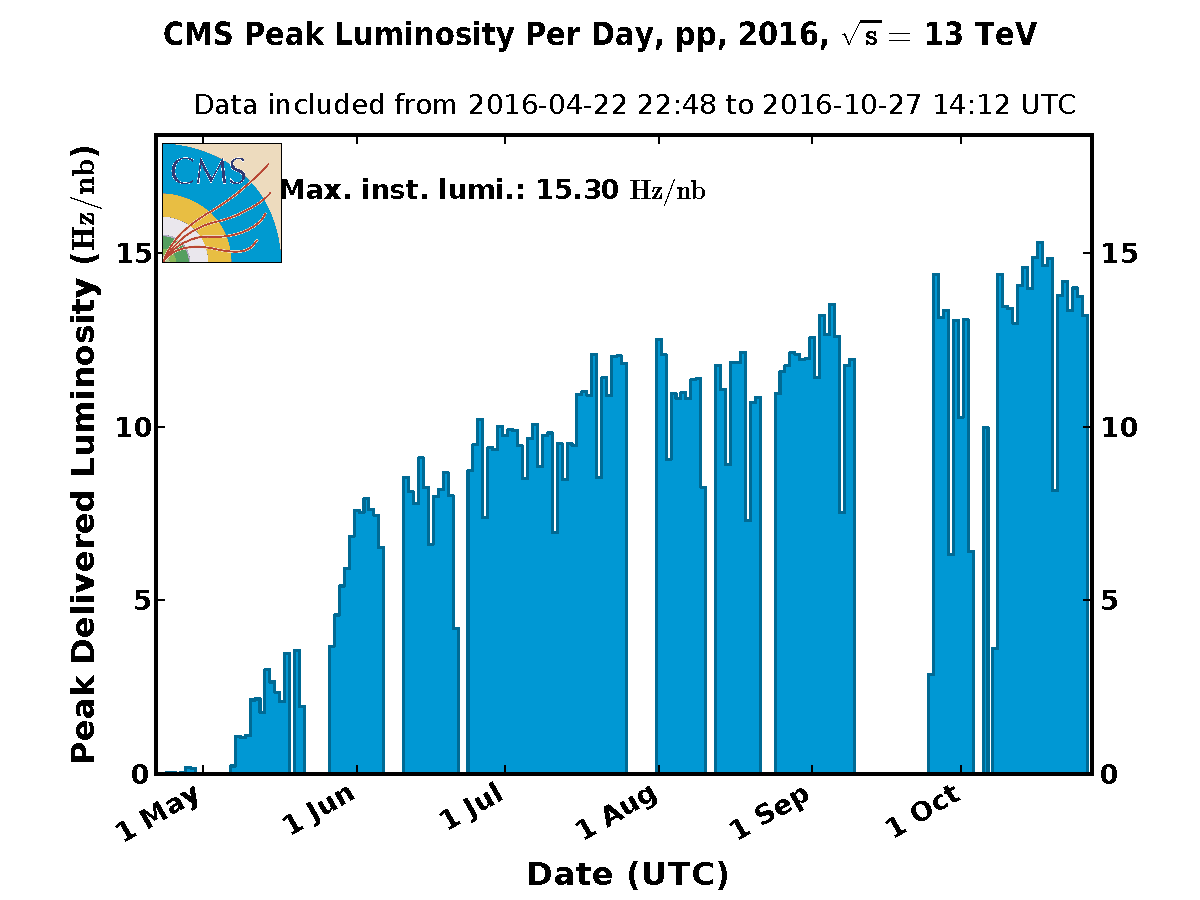
\includegraphics[width=.48\textwidth]{figures/peak_lumi_per_day_pp_2016.pdf}
    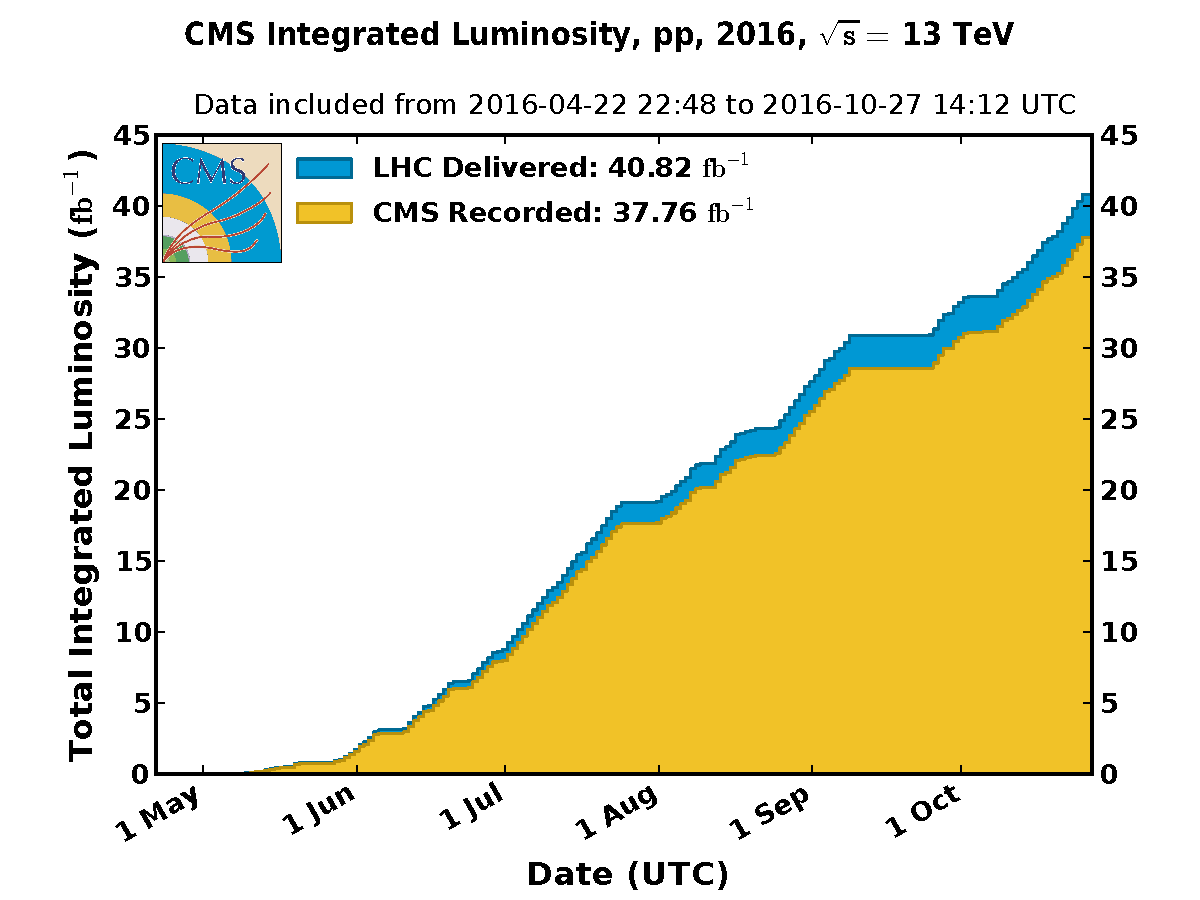
\includegraphics[width=.48\textwidth]{figures/int_lumi_per_day_cumulative_pp_2016.pdf}
    \caption{Peak instantaneous and integrated luminosity over time during the 2016 LHC proton-proton run delivered to the CMS detector. The difference between the 35.9 fb$^{-1}$ used in this analysis and the shown 37.76 fb$^{-1}$ comes from the omission of certain run periods where the detector was not operating optimally for the detection of leptons. Taken from \cite{lumi_twiki}.}
    \label{fig:lumi_stats}
  \end{figure}

  \subsection{What gets made?} \label{sec:what_gets_made}
    As mentioned in the previous section, the typical number of collisions leading to measurable energy deposits in the detector is 20 per bunch crossing. Figure \ref{fig:lhc_decay_modes} shows cross section for various proton-proton final states as a function of center of mass energy. Notice that the vast majority of the collisions result in low energy jet production or elastic scattering. 

    The analysis presented in this thesis is concerned with the production of Z bosons, whose production cross section is denoted as $\sigma_\text{Z}$ in the figure. Given the instantaneous luminosity of $10^{34}$ cm$^{-2}$ s$^{-1}$, the production cross section corresponds to a rate of 1000 Z bosons produced per second at peak luminosity. Given the total integrated luminosity of 35.9 fb$^{-1}$, the entire CMS dataset during this time period contained approximately 300 million Z bosons.

    Notice that the vast majority of collisions create only colored particles in the prompt process. Therefore, the most likely effect of the extra 20 collisions in a bunch crossing is to produce soft hadronic jets. For instance, the chance to produce another Z boson in an event that already has a Z boson is roughly 20 in a million, or 1 in 50,000. However, it is still important that particles from other collisions do not contaminate an event. As will be discussed more thoroughly in section \ref{sec:vertex_selection}, charged particle tracks can be traced back to the beamline and clustered into points of origin called a verticies. The vertex that is assigned the most total energy in an event is called the primary vertex. The chance that two high energy verticies will exist in a single event is low since the number of collisions per crossing is small compared the ratio of the cross section of interesting physics to the total proton-proton cross section.


    \begin{figure}[h!]
      \centering
      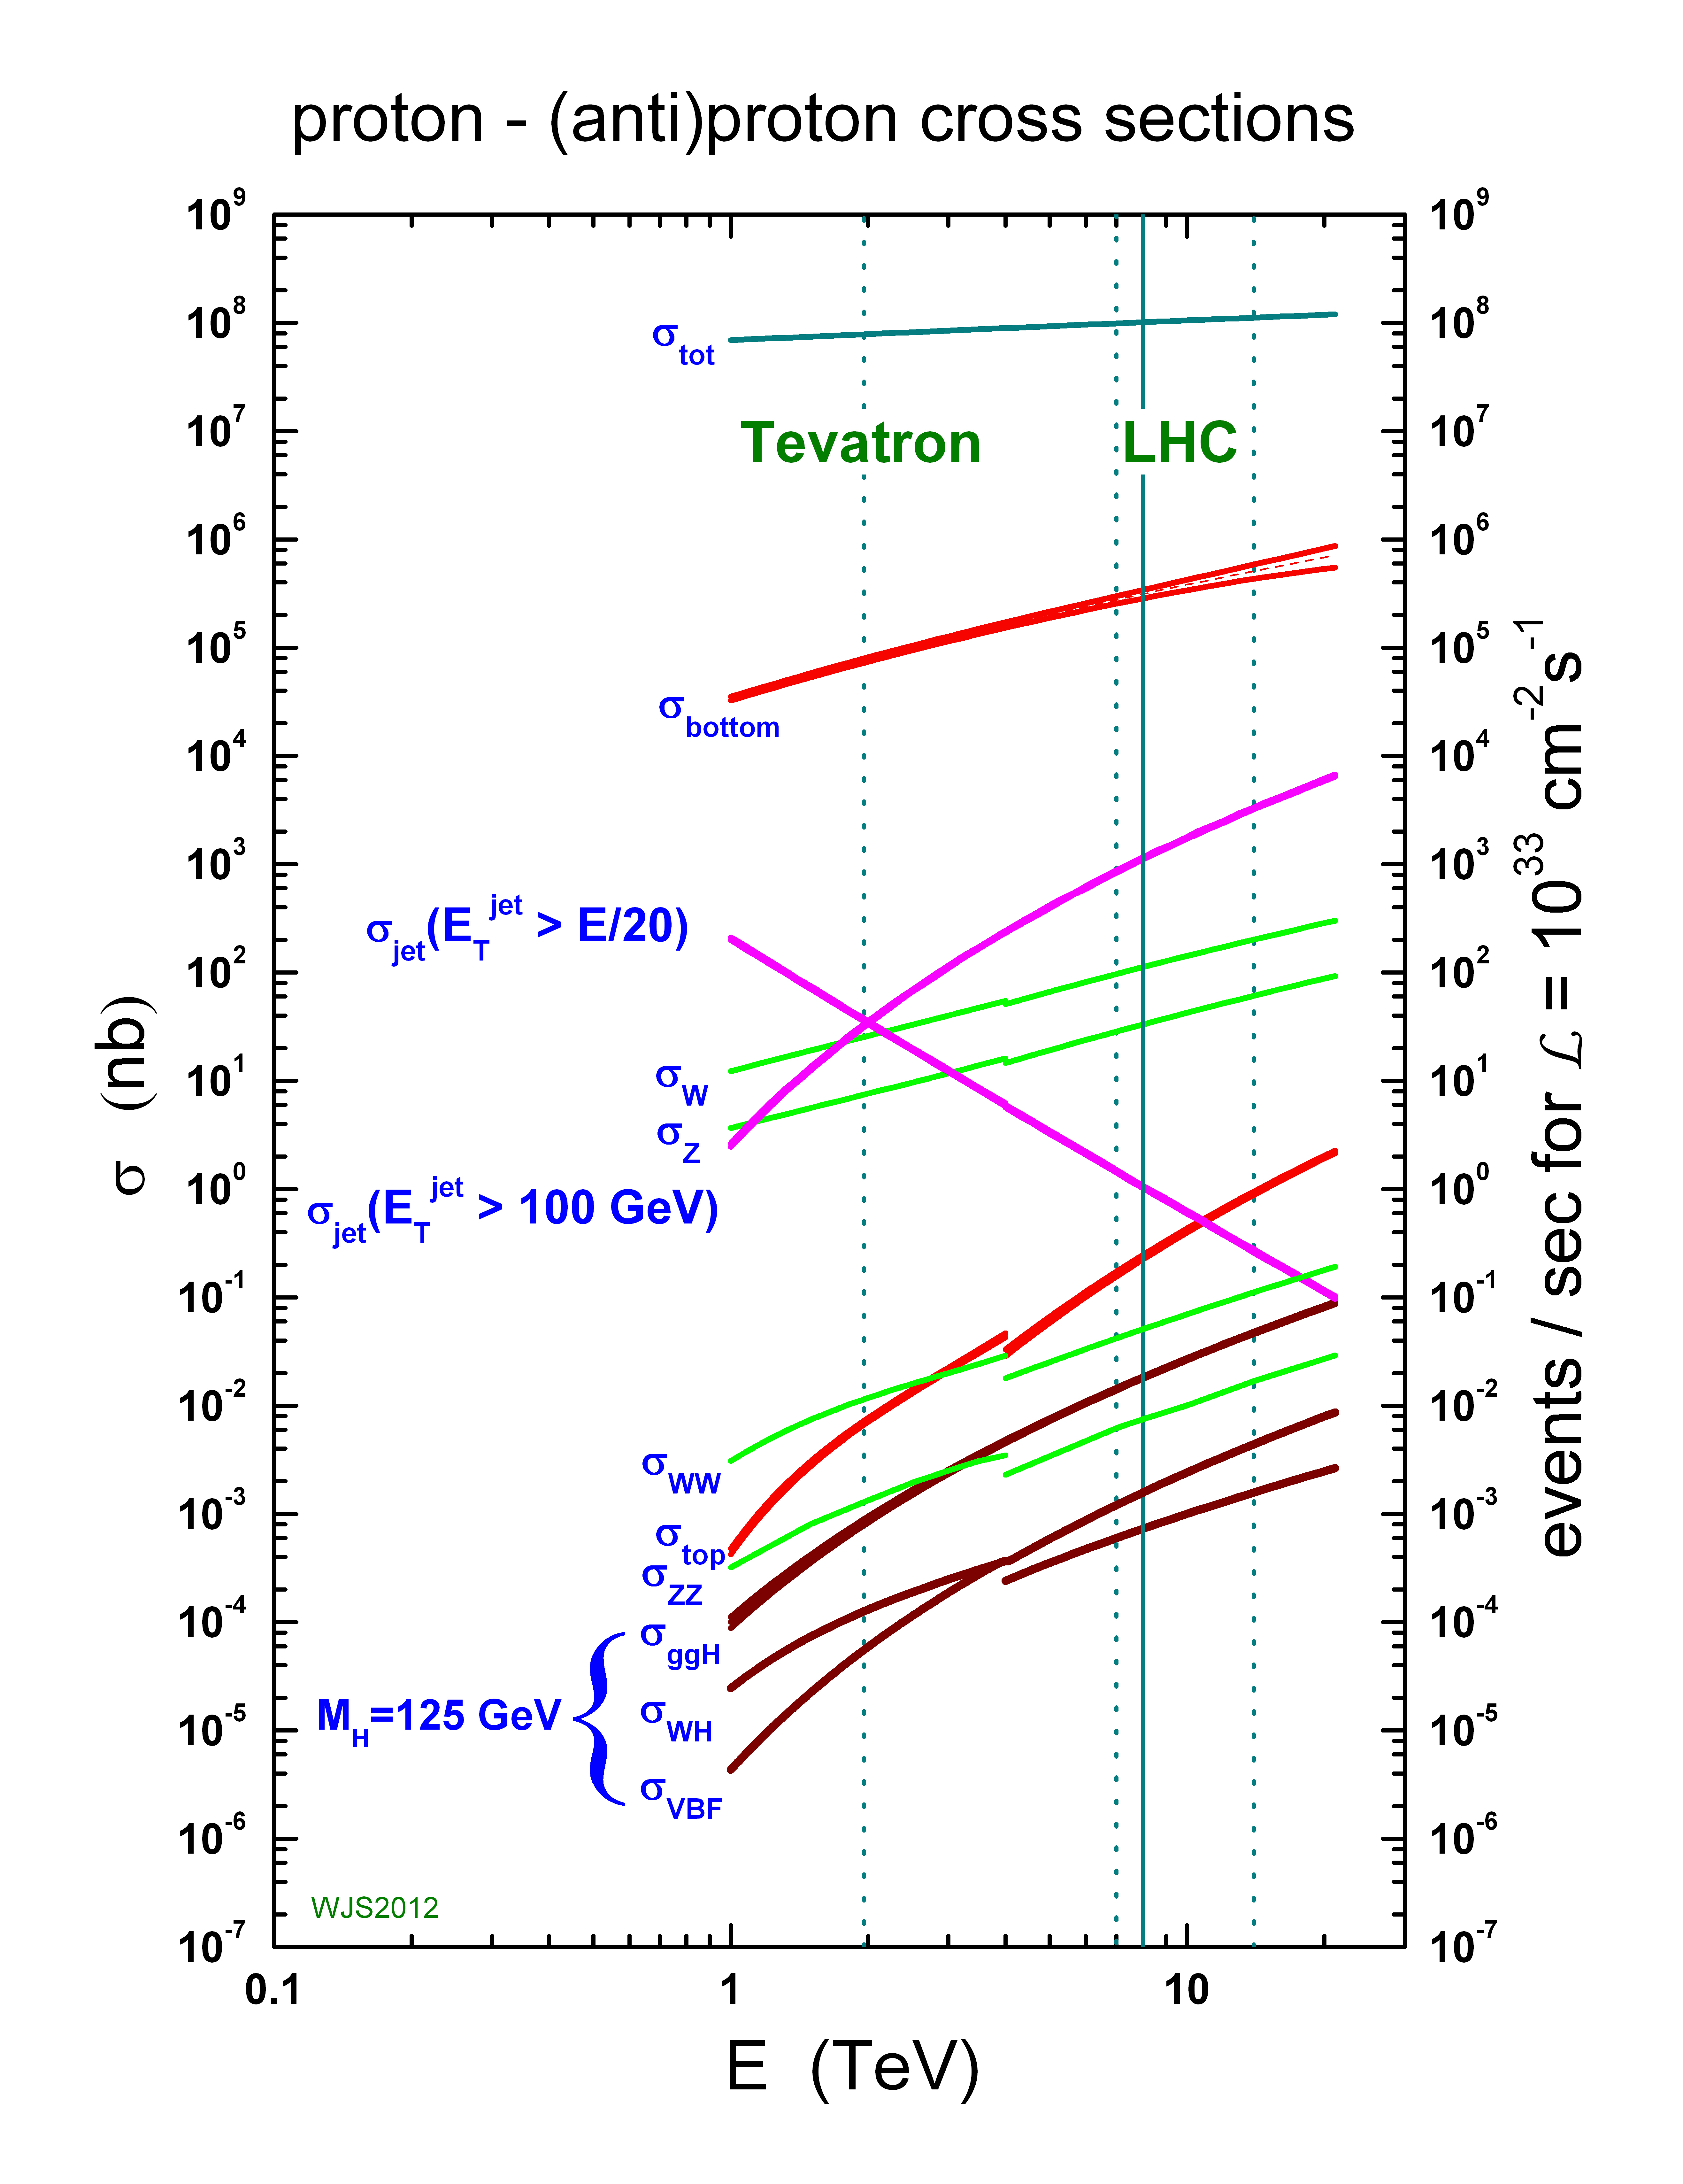
\includegraphics[width=.7\textwidth]{figures/lhc_decay_modes.jpg}
      \caption{Production Cross Sections for proton-proton collisions. Cross sections at center of mass energy less than 4 TeV are taken from proton-antiproton collision data at the Tevitron, which leads to some discontinuity for some types of electroweak boson production.}
      \label{fig:lhc_decay_modes}
    \end{figure}

    \begin{figure}[h!]
      \centering
      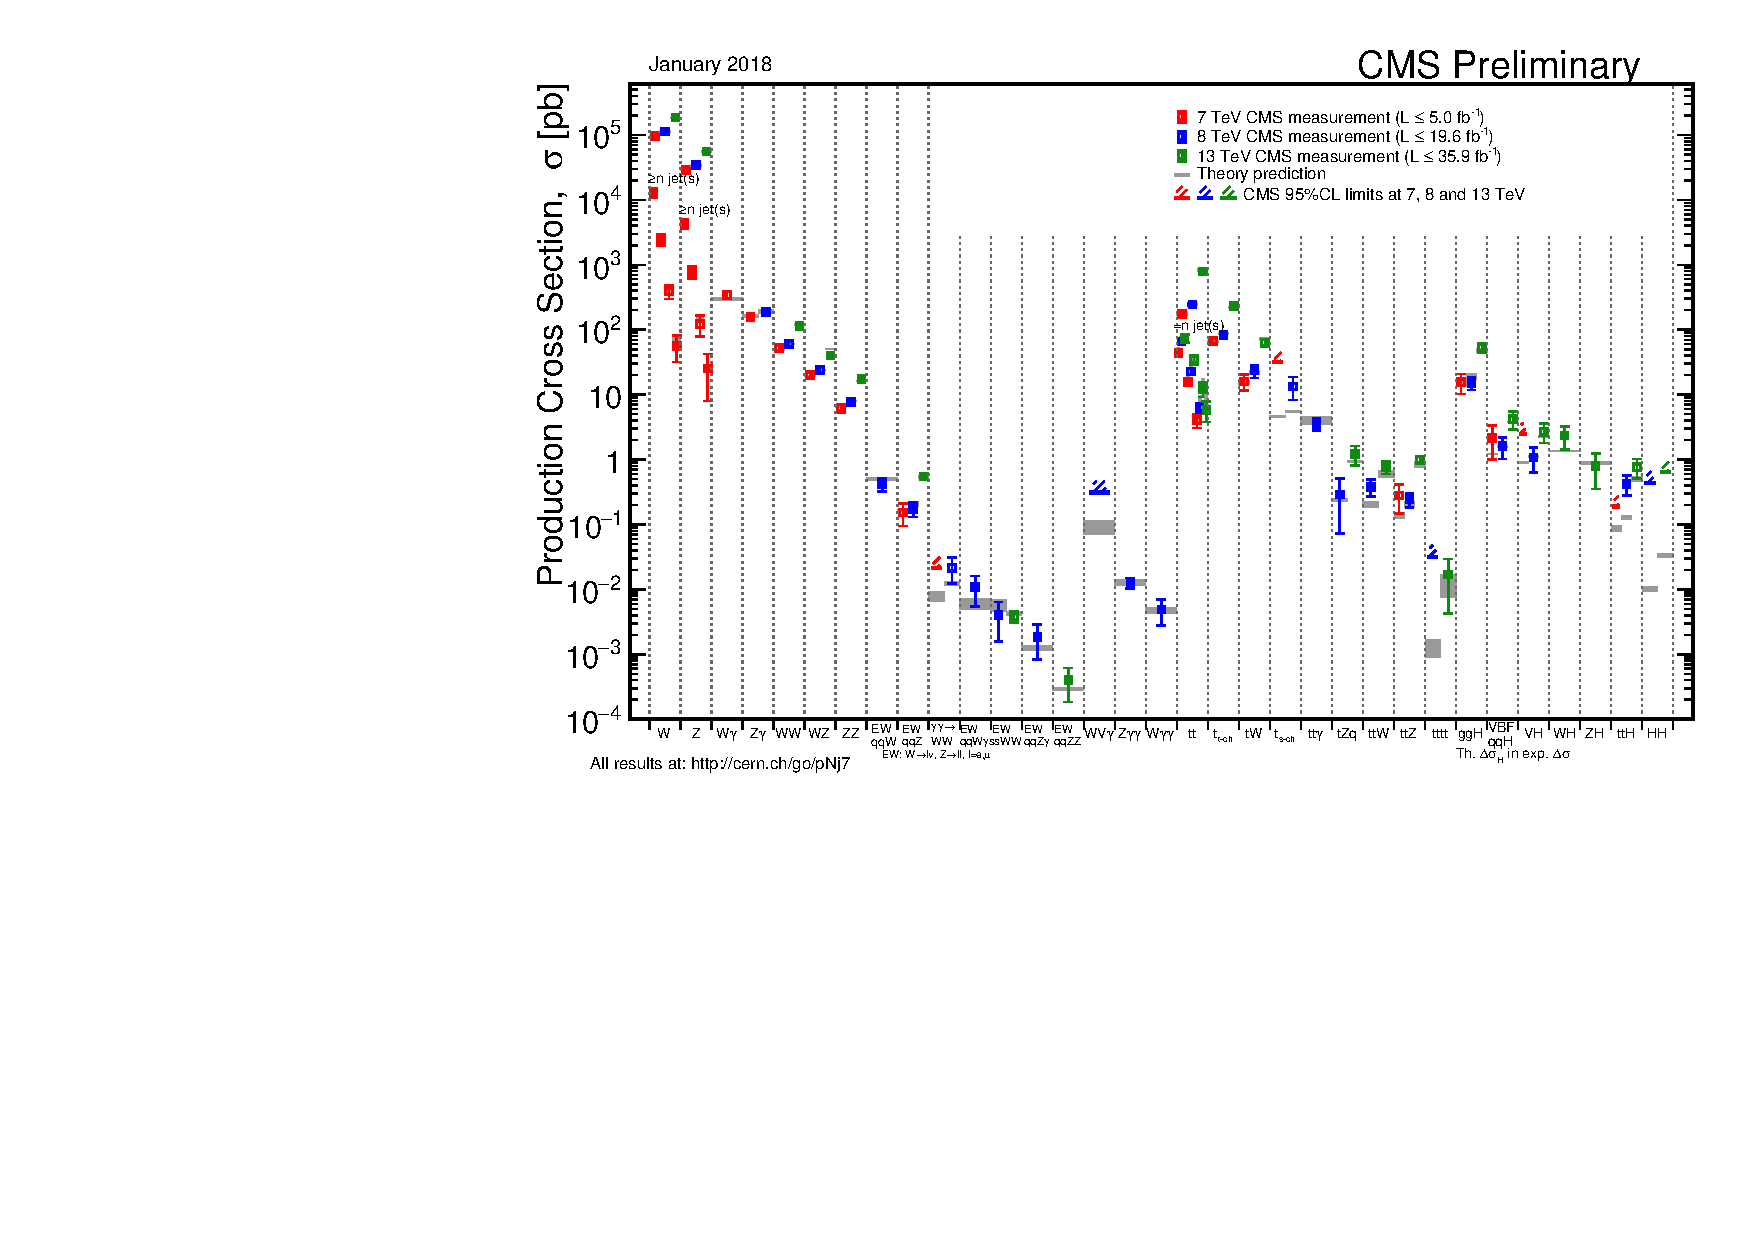
\includegraphics[width=.7\textwidth]{figures/cms_cross_sections.pdf}
      \caption{Cross sections measured by the CMS collaboration as of January 2018. Note that the cross section for Z+2 jets is close to the cross section for TTBar production. Additionally, note that for W and Z bosons, the cross section reduction in adding an additional jet is a factor between 5 and 10, consistent with the value of $\alpha_s$ at these energies. Taken from \cite{cms_results}}
      \label{fig:cms_cross_sections}
    \end{figure}

    \todo{Point out that there is very low chance for double scattering or two interesting interactions in one bunch crossing. 
    Point out cross section of Z boson, point out the NJets rule.
    Consider adding the other figure on my wall at the office. That way I can point out the njets rule and show the background composition with 2 jets.}

\section{The CMS Detector}
  
  The Compact Muon Solenoid (CMS) is a general purpose detector at the LHC. The detector is shown in figure \ref{fig:cms_detector}. It is the second largest detector at the LHC, weighing just under 15 kilotons. The envelope of the detector is a cylinder of radius 7.3 meters and length of 21.6 meters. The detector subsystems are embedded like an onion, sorted by what a particle produced at the interaction point would encounter traveling away from the beam pipe, the detector subsystems are as follows:

  \begin{enumerate}
    \item{Silicon Pixel Tracker}
    \item{Silicon Strip Tracker}
    \item{Electromegnetic Calorimeter}
    \item{Hadronic Calorimeter}
    \item{Superconducting Solenoid}
    \item{Muon Drift Tubes}
  \end{enumerate}

  The subsystems are broken into at least two regions. The \emph{barrel} region is the central part of the detector, and it is built of mostly of detection modules that are oriented parallel to the beam pipe, since particles traveling through this part of the detector have more transverse than longitudinal momentum. The \emph{end cap} contains modules oriented perpendicular to the beam pipe, since particles traveling through this part of the detector have more longitudinal momentum.

  \begin{figure}[h!]
    \centering
    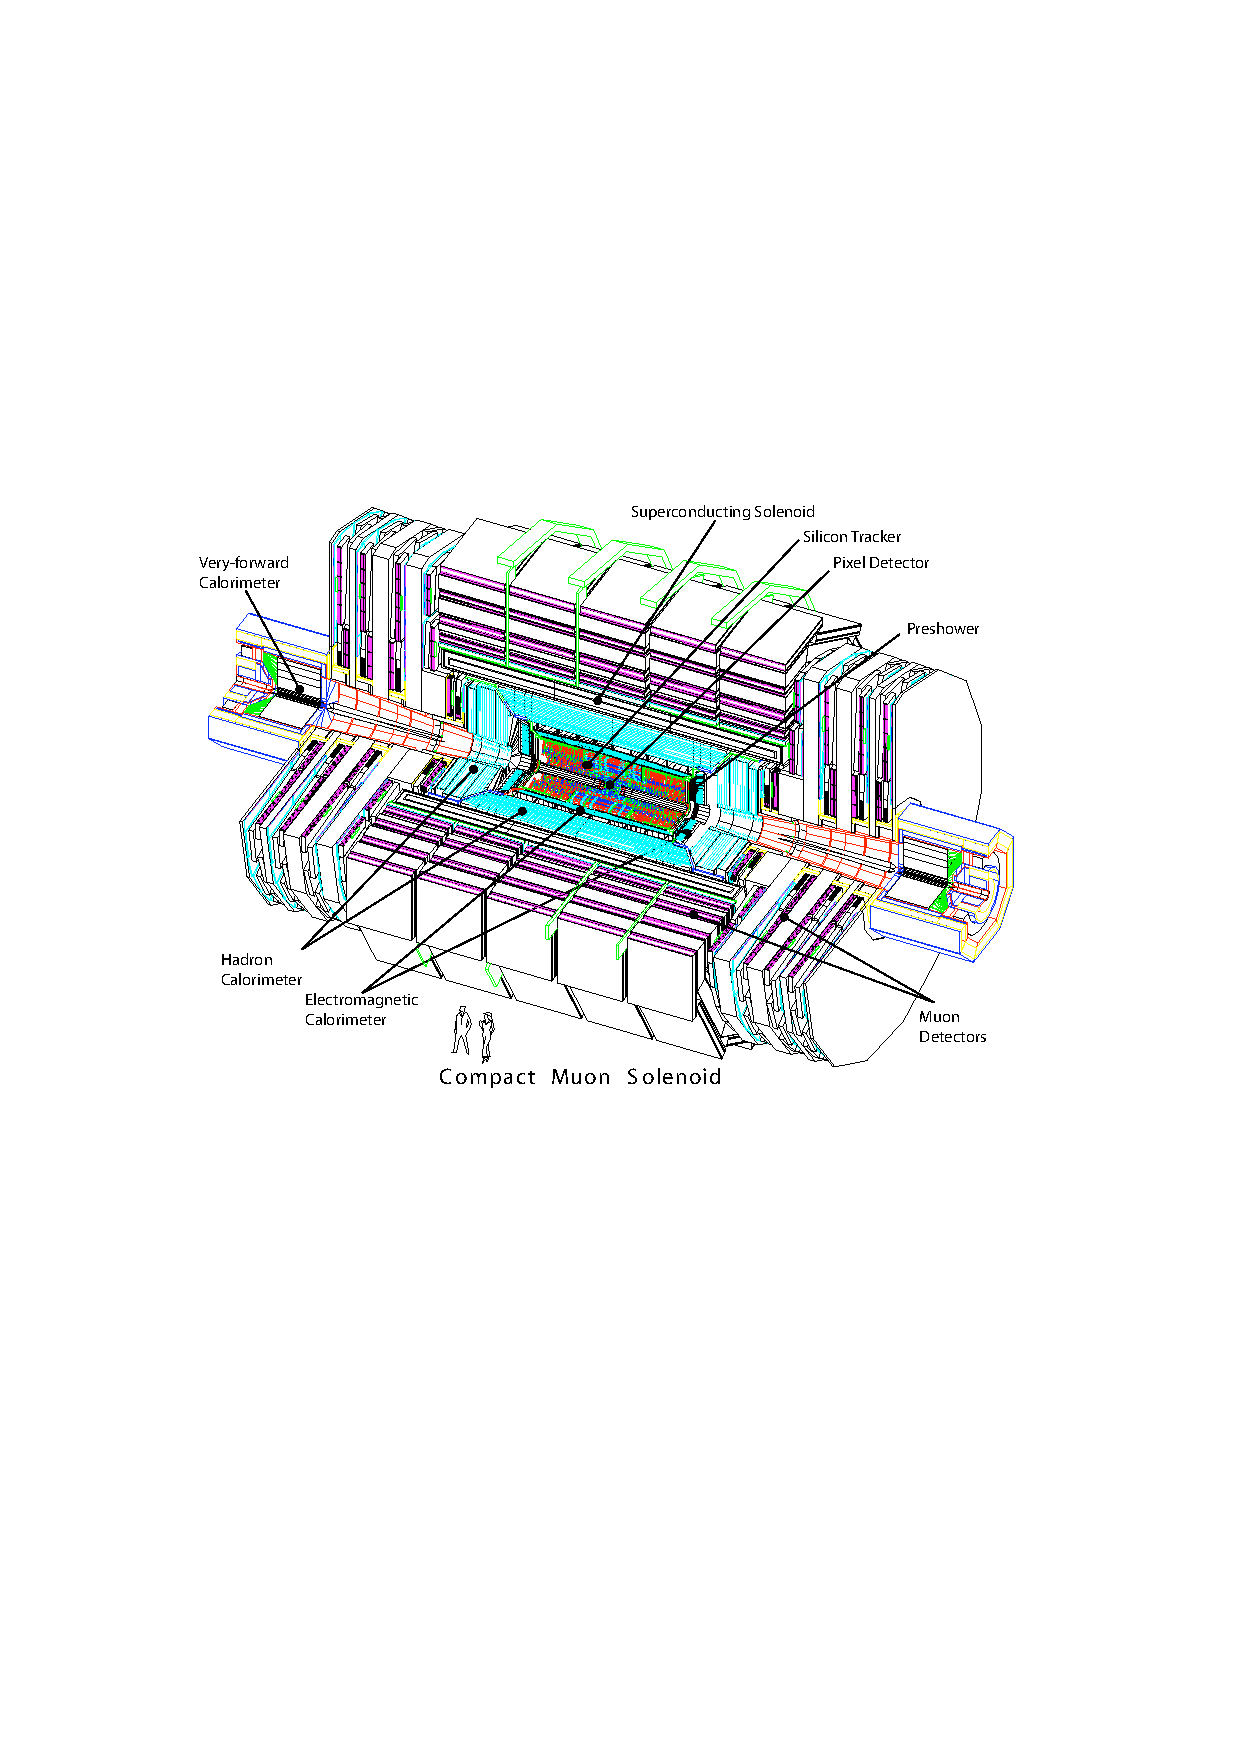
\includegraphics[width=.7\textwidth]{figures/cms_detector.pdf}
    \caption{A cutaway drawing of the Compact Muon Solenoid. Taken from the CMS TDR \cite{cms_tdr}.}
    \label{fig:cms_detector}
  \end{figure}

  As was shown in sec \ref{sec:what_gets_made}, most collisions at the LHC produce sprays of hadrons called jets, in fact the bulk of interactions are between gluons. However, more rare electroweak processes, such as the production of the higgs boson, can lead to the creation of leptons. Therefore, measuring the energy spectra of leptons is of central importance for CMS analyses searching for new physics coupled to the electroweak sector; this search is one such analysis. 

  The CMS detector needs to be able to identify charged leptons and distinguish their flavor in order to probe electroweak physics without hadronic backgrounds. The electron is a stable particle, and the muon has a lifetime long enough that it should make it through

  In order to measure the momentum of charged particles, a large magnetic field is applied by a superconducting solenoid that is placed between the hadronic calorimeter and the muon system. The solenoid creates a roughly constant 3.8 Tesla magnetic field parallel to the beam pipe in the region of the detector filled by the tracking system and calorimeters. This magnetic field will bend charged particles in accordance with the Lorentz force law and allow for a measurement of the particles momentum.

  CMS was designed with several physics goals in mind, from finding the Higgs boson, to searches for dark matter and supersymmetry. The technical design report (TDR) \cite{cms_tdr} summarizes the physics and design goals for the detector. A short list follows:

  \begin{enumerate}
    \item The search for the Higgs boson, specifically in the dimuon and diphoton channel\footnote{the diphoton channel was where it ultimately was found}. This created a need for excellent muon and photon energy resolution and isolation. These requirements justify the advanced muon system and ECAL. Additionally searching for the Higgs in the $b\bar{b}$ and $\tau \bar{\tau}$ channels created the requirement for good offline b-tagging and $\tau$-tagging capabilities, largely regulated by tracker resolution.
    \item The search for supersymmetric (SUSY) particles. The main motivation for these searches is often in the context of R-parity conserving SUSY due to the natural dark matter candidate they provide as described in section \ref{sec:r-parity}. Dark particles leave momentum imbalance in the detector, so there is 
    \item The search for new massive vector bosons, typically dubbed a Z' search. Here dilepton (electron and muon) energy resolution are again of the paramount importance.
    \item The search for extra dimensions. The phenomenology of these models is very broad, but signatures can include all massive standard model particles and gravitons which leave a \MET signature.
    \item Measurements furthering the precision Standard Model parameters. The production of top quarks is enhanced at the LHC compared to any previous colliders due to their large mass, even compared to the TeV scale. Top quarks almost always decay to b-quarks which means the LHC is also a b-factory.
    \item In addition to proton-proton collisions, the LHC also collides lead ions which probe the thermodynamic properties of quantum chromodynamics (QCD), the theory of the strong nuclear force. These collisions typically produce hadronic jets and their \pt spectrum is of interest due to observations at RHIC \cite{QCD_collider_physics}.
  \end{enumerate}

  \subsection{Coordinate System}
    Throughout this document, a standard coordinate system is used, this system is a cylindrical coordinate system with the $z$ axis oriented along the beam pipe. $z=0$ is situated at the mid-point of the detector, 10.8 m from either edge. The $\theta = 0$ direction points toward the Jura mountains, with $\theta = 90^\circ$ pointing straight upwards, away from the center of the earth. 

    Rather than $\theta$, we use the pseudorapidity, $\eta = - \ln \left( \tan\left(\frac{\theta}{2}\right)\right)$. $\eta = 0$ corresponds to $\theta = 90^\circ$ and $\eta$ grows to infinity as $\theta$ goes to 0. The benefit of using $\eta$ is that differences in $\eta$, $\Delta \eta$, between two particles are approximately invariant under Lorentz boosts along the beam axis, whereas differences in $\theta$ are not. The extent to which $\Delta \eta$ is equal in different reference frames is regulated by the mass of the particles, with equality achieved in the case where the mass to momentum ratio of the particles goes to 0, i.e. the high energy limit.\footnote{Pages 6-8 in reference \cite{psuedorapidity} shows that differences in rapidity are Lorentz invariant and that psuedorapidity and rapidity are equal in the high energy limit} The detector's fiducial area corresponds to about $\abs{\eta} < 2.4$, which is about $10^\circ$ off of the beampipe. The positive $x$ axis is defined as pointing to the center of the circle outlined by the LHC, and the positive $y$ axis points towards the sky. The $\phi$ direction is the angle from the positive $x$ axis to the positive $y$ axis. Figure \ref{fig:cms_coordinates} shows this information visually.

    \begin{figure}[h!]
      \centering
      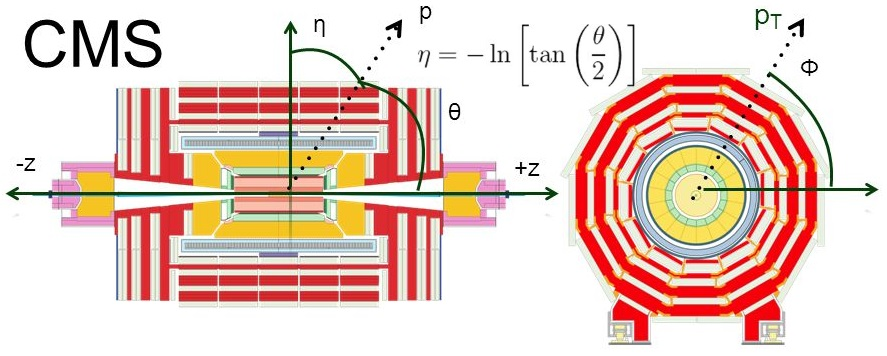
\includegraphics[width=.7\textwidth]{figures/cms_coordinates.jpg}
      \caption{Cross sectional and transverse views of the CMS detector with $\eta$, $\phi$, and $\theta$ coordinates shown. Taken from \cite{cms_coordinates}.}
      \label{fig:cms_coordinates}
    \end{figure}

  \subsection{The Inner Tracker} \label{sec:inner_tracker}
    The inner tracker is the closest part of the CMS detector to LHC beamline and interaction point where protons collide. \cite{cms_jinst} It surrounds the interaction point with a length of 5.8m and radius of 1.25m. The purpose of the system is to track charged particles to their vertex and measure the momentum of charged particles via the saggita in the particle arc due to the magnetic field. The entire active detection area of the inner-tracker system is made of silicon, but can be broken into 2 main subsystems:

    \begin{enumerate}
      \bitem{pixel detectors} The innermost part of the tracker system is a pixel-based detector composed of 1,440 thin modules, of cross section $100 \times 150 \mu$m$^2$, capable of measuring hits with fine granularity in 3 dimensions. This subsystem's main purpose is to aid in vertex reconstruction.
      \bitem{strip detectors} The outer part of the inner tracker is composed of 15,148 strip modules. The main purpose of this subsystem is to track charged particles from the vertex into the ECAL and also to give one measure of their momentum.
    \end{enumerate}

    Silicon detectors work on the principle of semi-conduction. When a charged particle passes through the material, electrons are kicked into the conduction band and drift, due to a bias voltage applied across the sample, towards electronics attached to the material that record the current. Because silicon has a relatively small band gap, the entire tracking system needs to be kept at low temperature, approximately $-10^\circ$ C, in order to keep the electrons stationary in the valence band in the presence of the bias voltage.

    The tracker geometry is shown in figure \ref{fig:strip_tracker_geometry}. The pixel detectors are the closest to the beampipe and consist of 3 layers in the barrel region and 2 annuli in the endcap region. The three barrel layers are positioned in concentric cylinders about the beampipe at radii of 4.4 cm, 7.3 cm, and 10.2 cm respectively. The endcap annuli are placed at $\abs{z} = 34.5 $cm and 46.5 cm respectively and have an inner radius of 6 cm and an outer radius of 15 cm. The strip tracker consists of an inner barrel region (TIB), an outer barrel region (TOB), and an inner disk region (TID) in the barrel, and two endcap regions (TEC +/-). 

    \begin{figure}[h!]
      \centering
      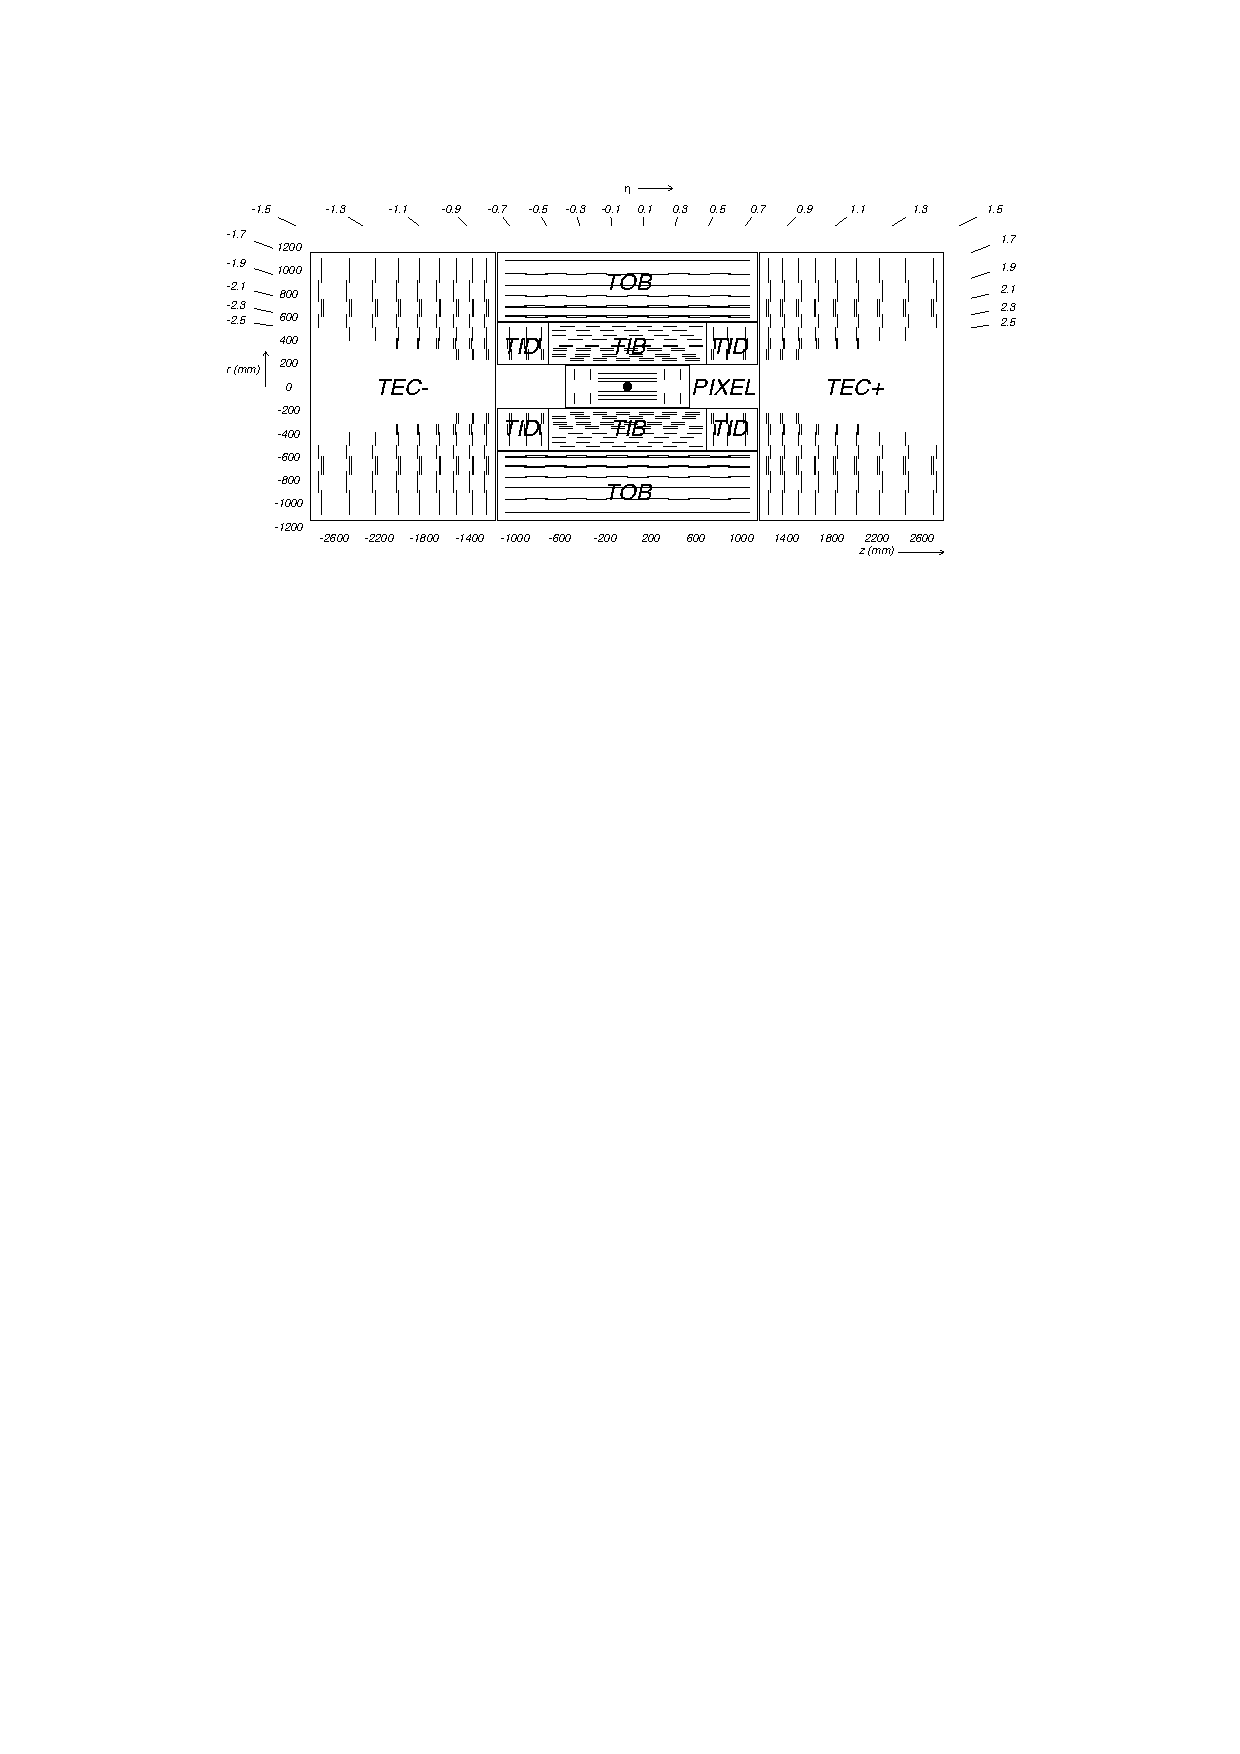
\includegraphics[width=.7\textwidth]{figures/cms_tracker_schematic.pdf}
      \caption{Schematic view of the CMS inner tracking system. Notice the detectors only cover $\abs{\eta}$ ranges less than 2.5 and that particles traveling near $\abs{\eta}=1.5$ pass through the most material. Taken from \cite{cms_jinst}.}
      \label{fig:strip_tracker_geometry}
    \end{figure}

    Because one of the goals of the tracking system is to obtain a measure of momentum by tracking the natural motion of particles through space in a magnetic field, it is important that the interactions between charged particles and the tracking system do not change the motion, and likewise the energy, of the particles dramatically. For particles other than the electron and photon, the silicon tracker has mostly negligible effects on the energy as the amount of bremsstrahlung is inversely proportional to the mass of the particle to approximately the 6th power;\footnote{This can be seen in the classical theory of bremsstrahlung radiation as described in \cite[pg. 464, eq. 11.75]{griffiths_em} by replacing the Lorentz factor $\gamma$ with $\frac{E}{mc^2}$. In the case of an acceleration in an orthogonal direction, $\gamma^6 \to \gamma^4$.} their main energy loss mechanism is through ionization.\cite[sec. 33.2]{PDG} However, for the electron and the photon, interaction with the tracker can cause bremsstrahlung radiation and pair production respectively.

    To understand the magnitude of these effects, it is typical to look at the number of radiation lengths\footnote{taken to be the distance at which a high energy electron is expected to lose $\frac{1}{e}$ of its energy \cite[sec 34.4.2]{PDG}, or $\frac{7}{9}$ the mean free path for a high energy photon.} of material in the tracker. The ``material budget" of the tracker is shown in figure \ref{fig:tracker_material_budget}. Due to the large amount of non-sensitive material in the range $\abs{\eta} \in [1.4,1.6]$, leptons for this analysis are not considered in that range, as is explained in section \ref{sec:dilepton_selection}. As can be seen in the figure, many $\eta$ values correspond to high probability of radiation and pair production for electrons and photons respectively. We will explain in section \ref{sec:particle_flow} how the momentum of these types of particles is reconstructed given these issues.

    \begin{figure}[h!]
      \centering
      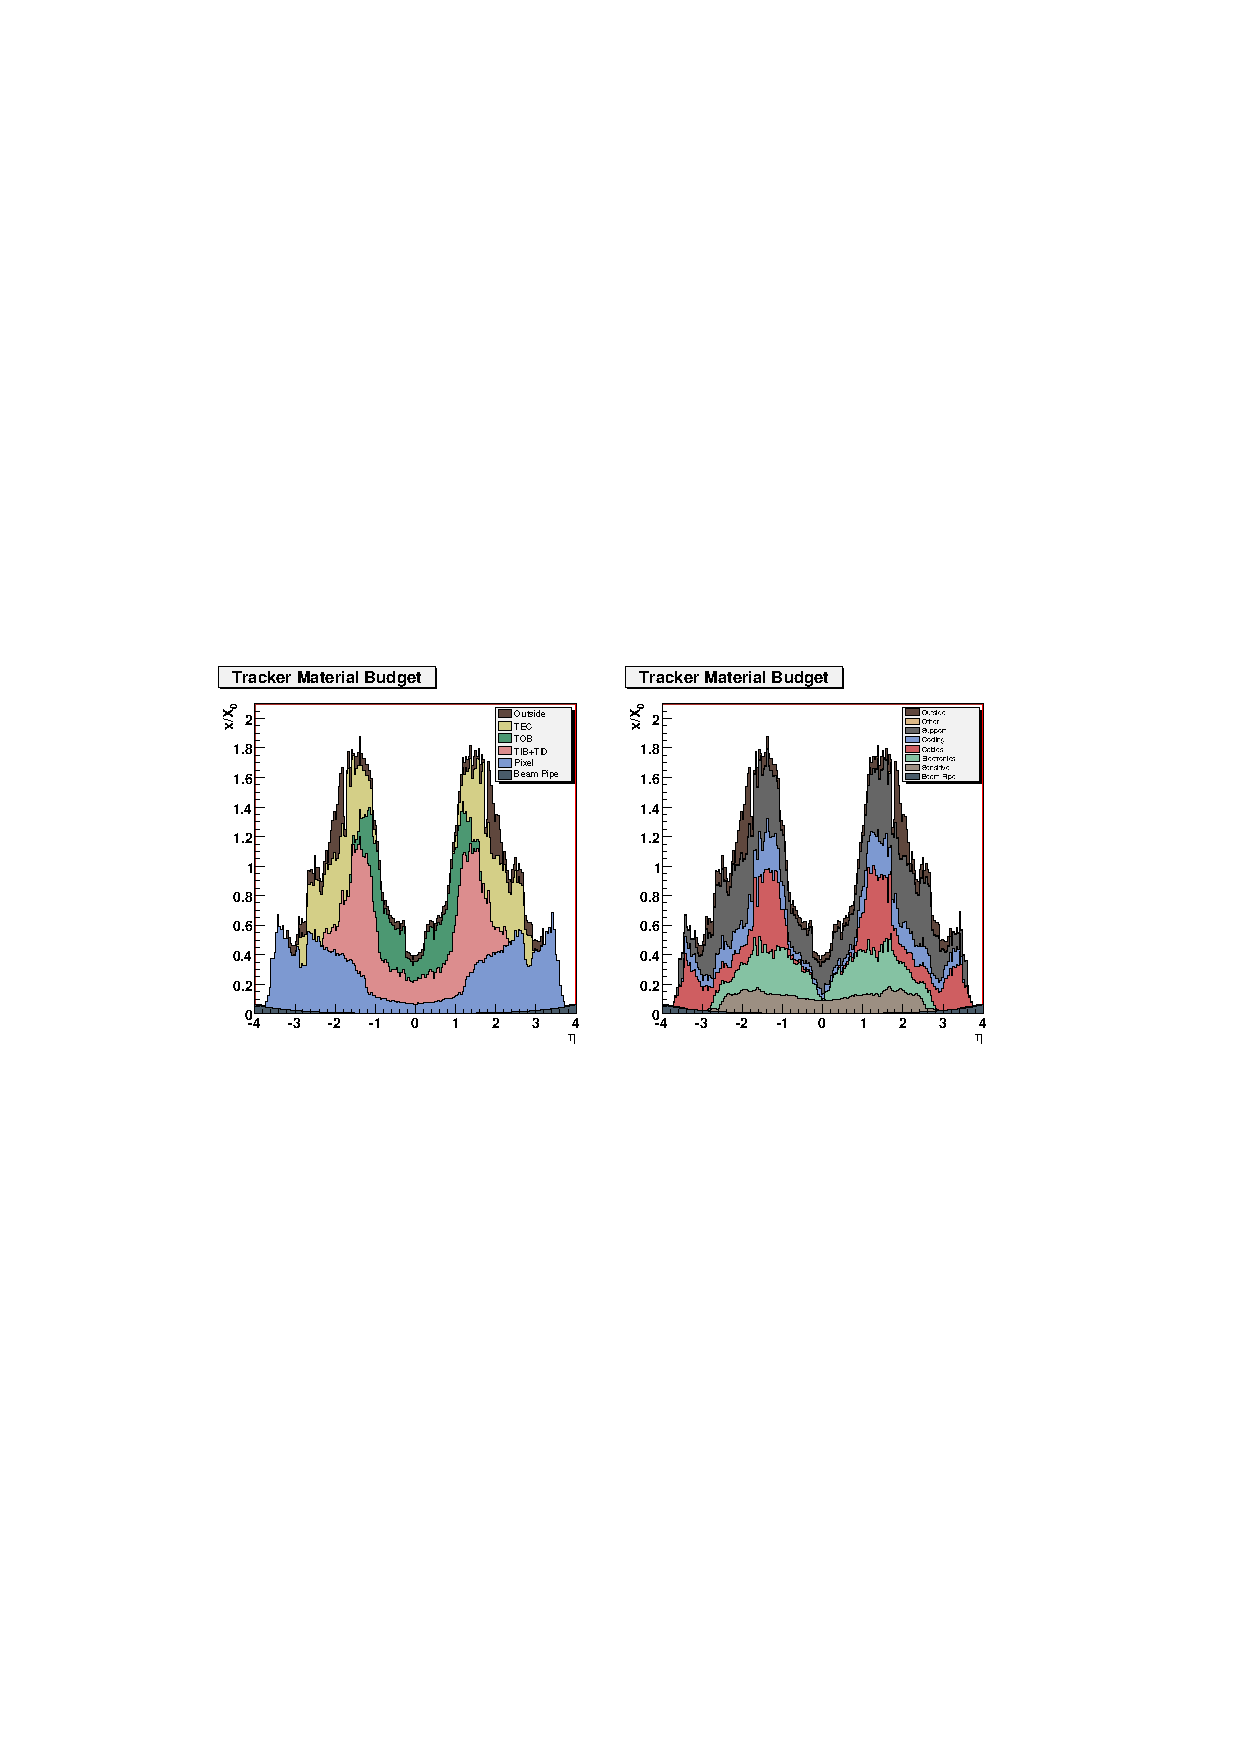
\includegraphics[width=.9\textwidth]{figures/cms_tracker_material_budget.pdf}
      \caption{The material budget of the tracking system in radiation lengths. On the left, the material is broken down by tracker subsystem, on the right it is broken down by the type of component. As can be seen on the right plot, a large amount in non-sensitive material, like cables and support structure, is found near $\abs{\eta}=1.5$. For this reason, leptons in this analysis are not used if they are found in the window $\abs{\eta} \in [1.4,1.6]$. Taken from \cite{cms_jinst}.}
      \label{fig:tracker_material_budget}
    \end{figure}

  \subsection{The Electromagnetic Calorimeter} \label{sec:ECAL}
    The CMS Electromagentic Calorimeter (ECAL) is a nearly hermetic and homogeneous cylinder made of lead tungstate (PbWO$_4$) crystals with attached light measuring devices. The crystals are ``truncated pyramids", roughly rectangles of approximately 23 centimeters in length that taper slightly, from 26x26 mm$^2$ to 22x22 mm$^2$ in the barrel\cite[pg. 4]{cms_ecal}, to accommodate the curved shape of the ECAL in the $\phi$ direction and the angle at which the crystals are oriented to face the interaction point.\footnote{the crystals have a 3$^\circ$ angle with respect to the line that connects their incident face to interaction point in both the $\eta$ and $\phi$ directions to allow for better coverage of the fiducial volume.} Schematic views of the ECAL can be seen in figures \ref{fig:ecal_xsec} and \ref{fig:ecal_cutaway}. As can be seen in the figures, the calorimeter is broken into two physical sections, the barrel region (EB) and the endcap region (EE). The preshower disk in front of the endcap region is immaterial for this search, but is there to help distinguish between neutral pions converting to a di-photon pair with small angle separation from a single high energy photon. 

    \begin{figure}[h!]
      \centering
      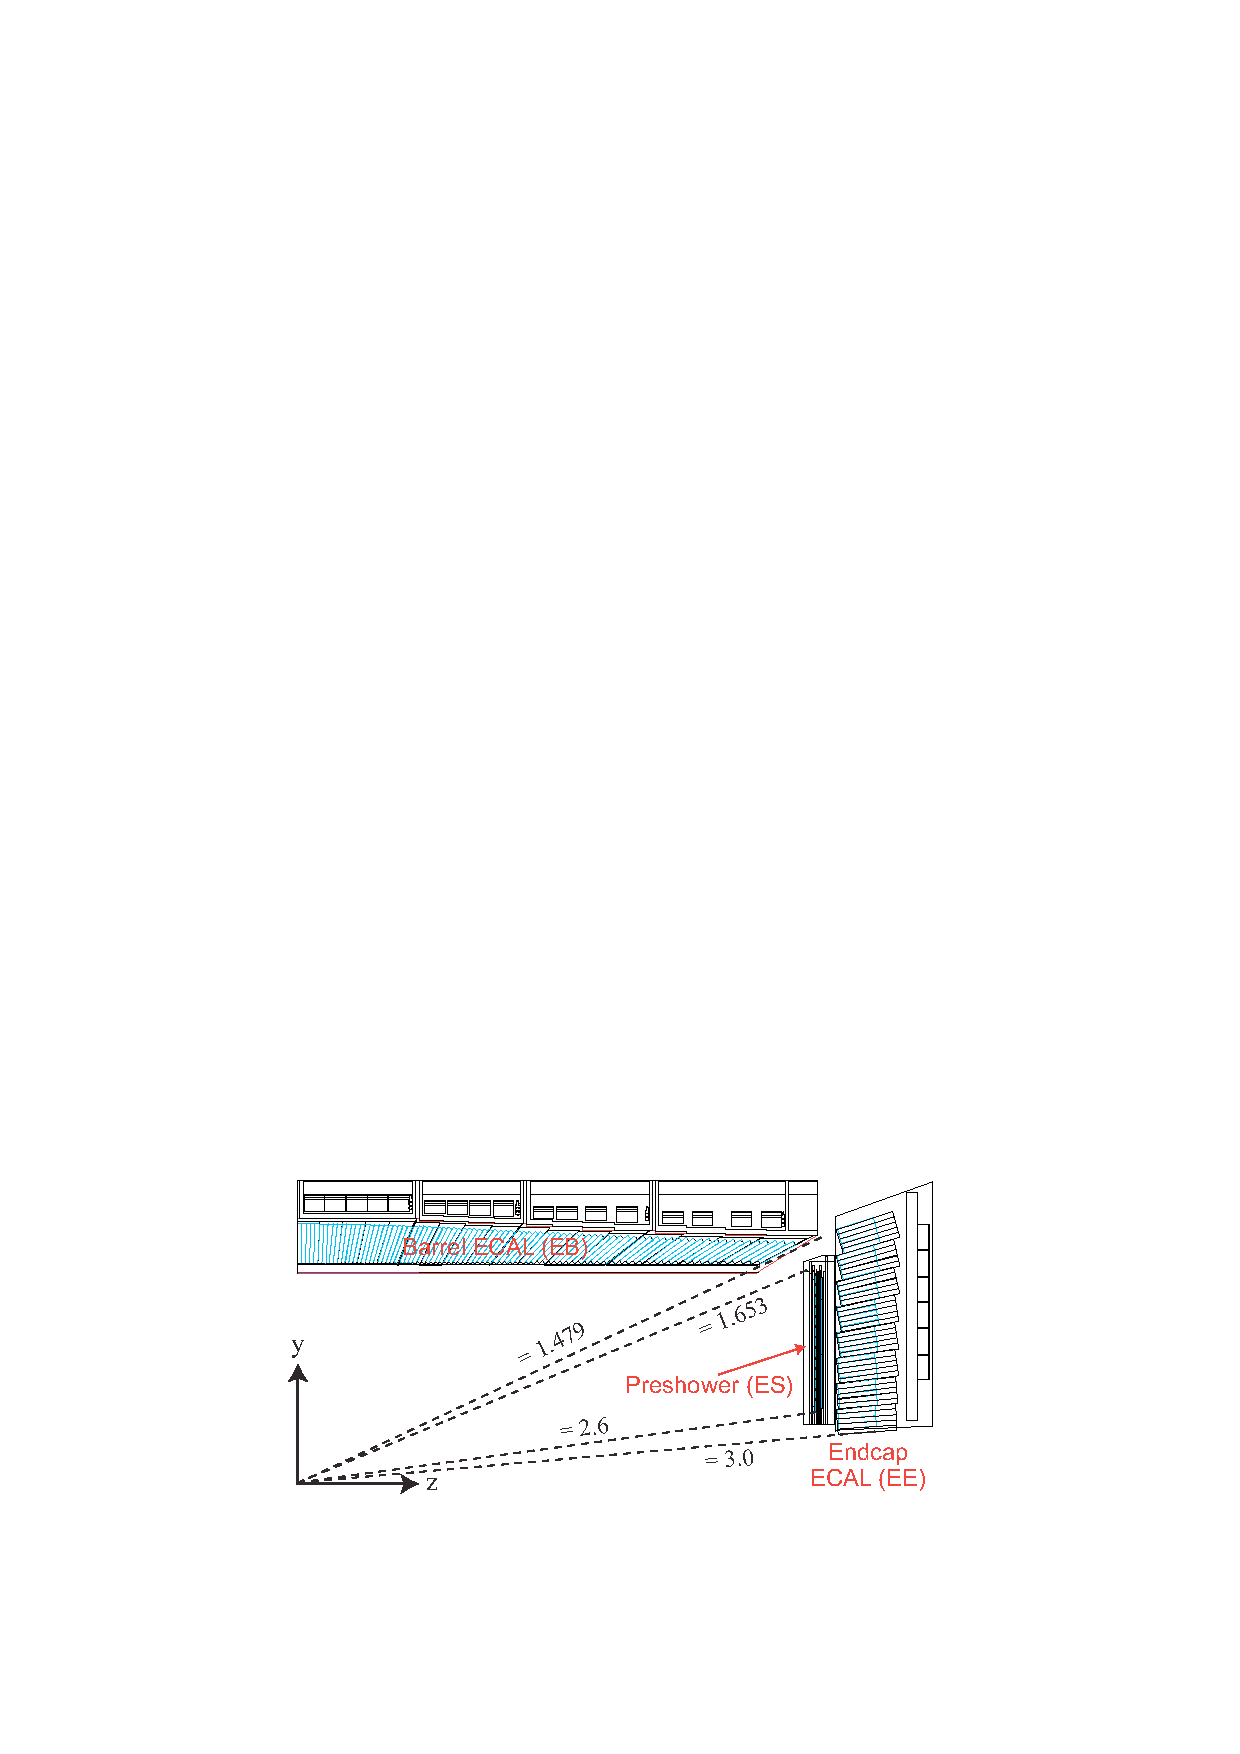
\includegraphics[width=.9\textwidth]{figures/cms_ecal_xsec.pdf}
      \caption{A cross sectional view of the electromagnetic calorimeter on the CMS detector. Notice the geometry of the crystals the transition region near $\abs{\eta} = 1.5$. Taken from \cite{cms_tdr}.}
      \label{fig:ecal_xsec}
    \end{figure}

    \begin{figure}[h!]
      \centering
      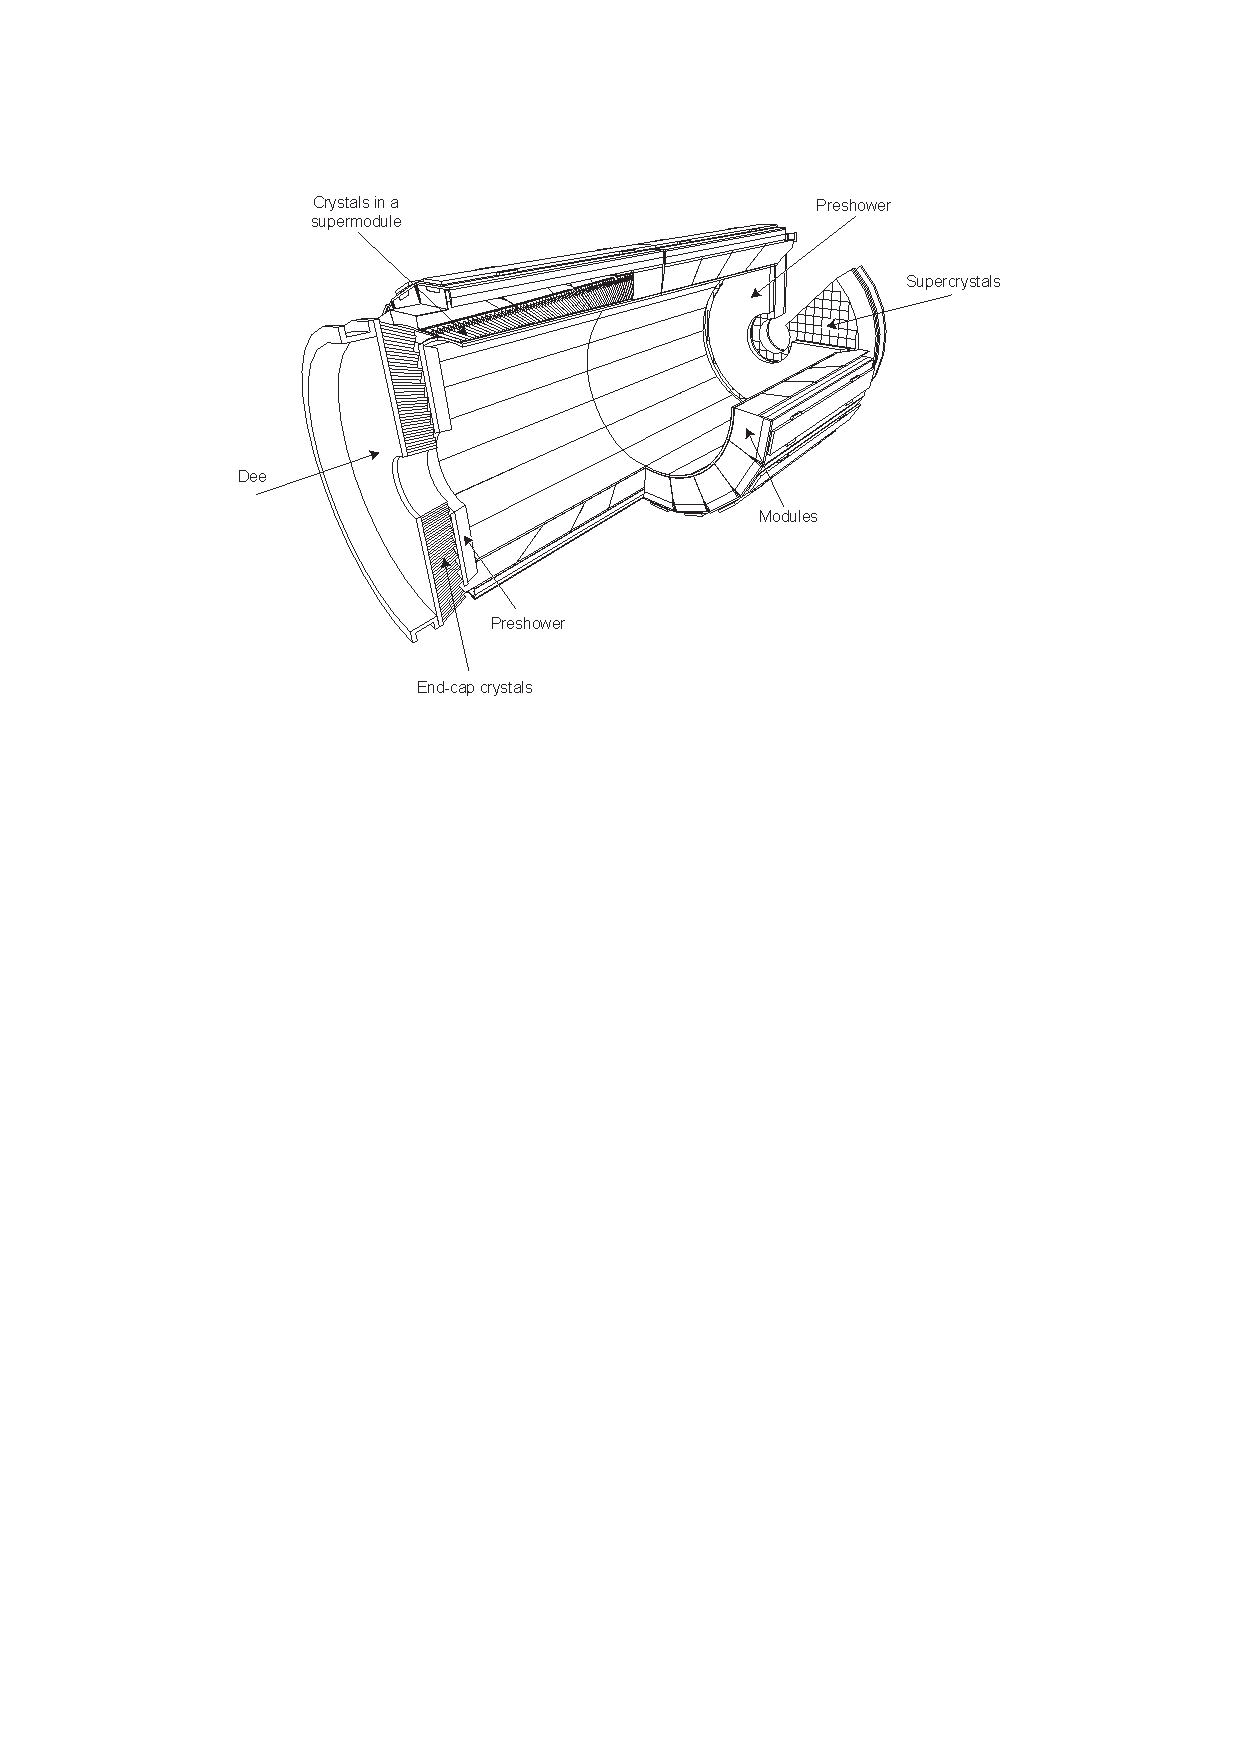
\includegraphics[width=.9\textwidth]{figures/cms_ecal.pdf}
      \caption{A cutaway of the electromagnetic calorimeter on the CMS detector. Taken from \cite{cms_jinst}.}
      \label{fig:ecal_cutaway}
    \end{figure}

    The purpose of the ECAL is essentially to give the most important measure of energy for electrons and photons. As explained in the previous section, the dynamics of electrons in material are quite distinct from heavier charged particles in material, the next lightest being a muon. Typical muon deposits in the ECAL are roughly 300 MeV\cite{muon_stopping_power}, whereas electrons under 500 GeV tend to have almost all of their energy absorbed by the ECAL\cite[sec. 4.10]{cms_jinst}. This is to say that charged particles heavier than an electron tend to pass right through the ECAL with little disturbance. \todo{Is this actually correct? Should I have a section somewhere where I describe charged particle interactions with matter?}

    The ECAL operates on the principle of scintillation\cite[ch. 7]{leo_detectors}, and makes use of the fast scintillation time (80\% of light emitted within 25 ns), high stopping power, and consequently small Moli\`ere radius of lead tungstate. The lead tungstate crystals have a length which corresponds to approximately 25 radiation lengths, this ensures that almost all of the energy carried by a high energy photon or electron will be radiated. The small Moli\`ere radius allows for good spacial resolution of energy deposits. \cite[pg. 90]{cms_jinst} Two things happen when an electron or photon is incident on one of the crystals:

    \begin{enumerate}
      \item A cascade of electrons, positrons, and photons is created. This is due to the effects discussed in the previous section, photons will pair produce electron-positron pairs. Electrons and positrons undergo bremsstrahlung radiation in material creating high energy photons. The result is that these processes feedback on each other and the multiplicity of particles explodes in the material creating an ``electromagnetic shower". A hypothetical shower imposed on an ECAL crystal is shown in figure \ref{fig:ecal_crystal}.

      \item Scintillation light is emitted by the lead tungstate due to interactions with charged particles and the light captured by the photo detectors attached to the crystal.
    \end{enumerate}

    \begin{figure}[h!]
      \centering
      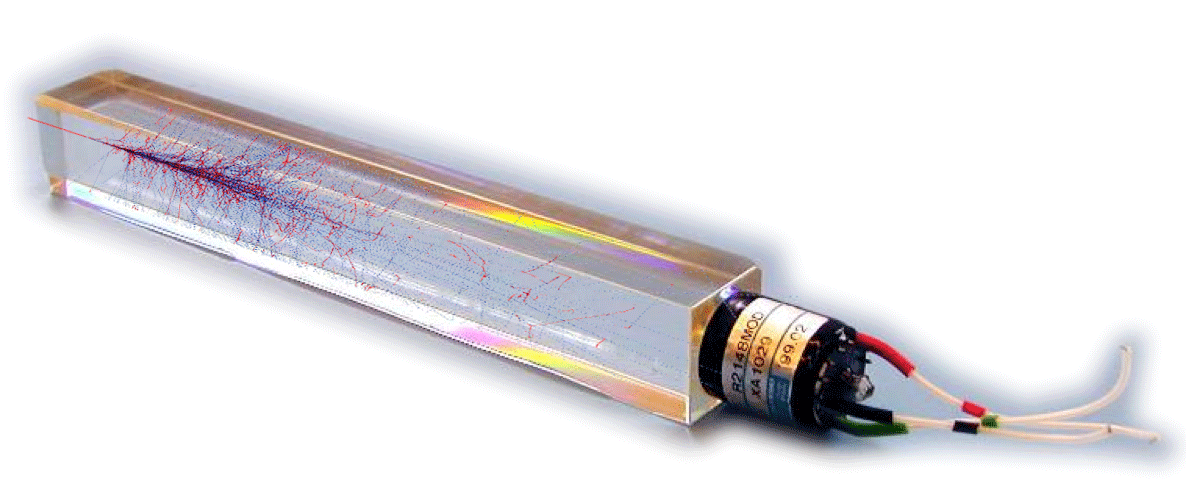
\includegraphics[width=.5\textwidth]{figures/cms_ecal_crystal_shower.png}
      \caption{A lead tungstate crystal from the CMS ECAL endcap region with a vacuum phototriode attached. A hypothetical shower from an electron is superimposed on the image. Taken from \cite{ecal_crystal}.}
      \label{fig:ecal_crystal}
    \end{figure}

    From the amount of scintillation light, the energy of the incident particle can be reconstructed with high resolution. Figure \ref{fig:ecal_resolution} shows the energy measured using a 5x5 grid of ECAL crystals for 120 GeV electrons. From the figure, we can see that the ECAL energy resolution is excellent for electrons in this range, the standard deviation of the energy measurement being 1-2\% of the energy.

    \begin{figure}[h!]
      \centering
      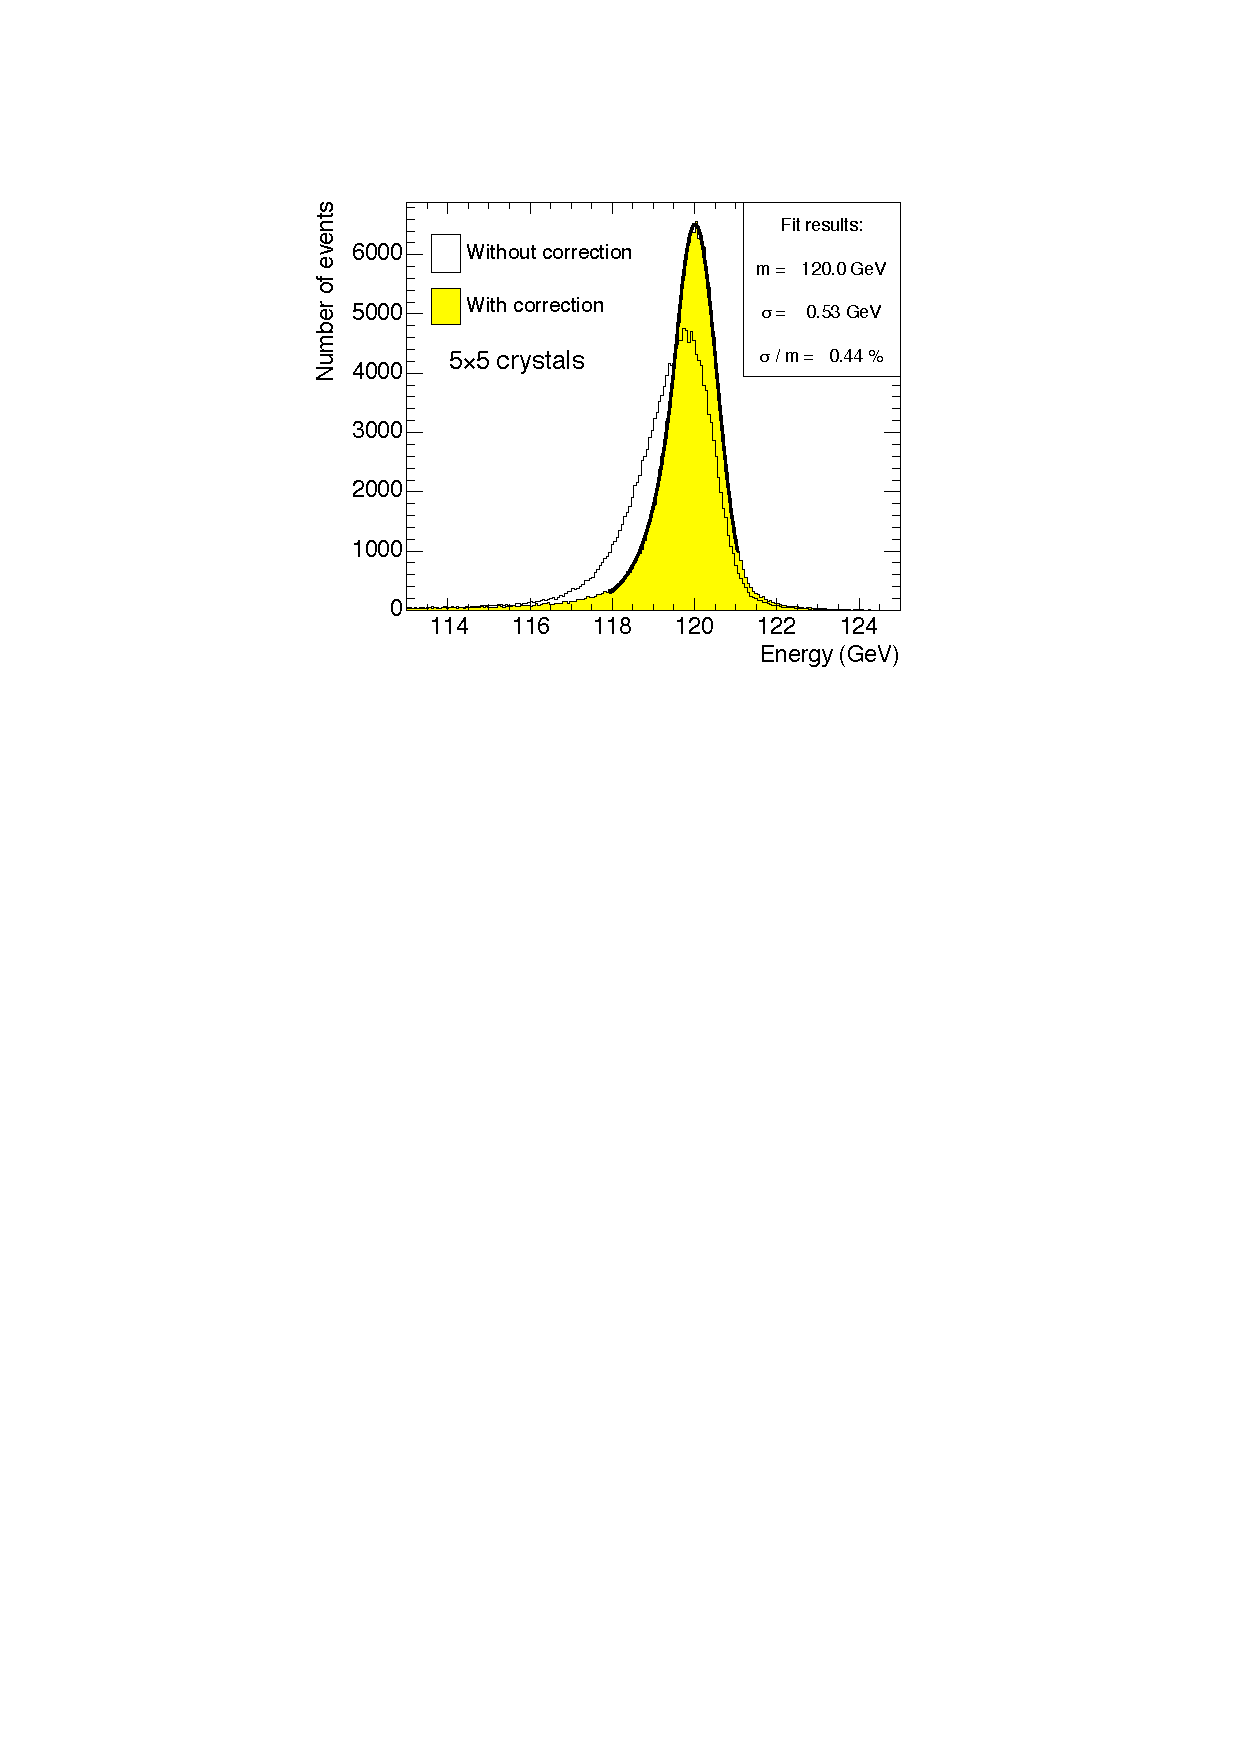
\includegraphics[width=.7\textwidth]{figures/ecal_resolution.pdf}
      \caption{The energy measured from 120 GeV electrons taken from a 5x5 grid of ECAL crystals. Taken from \cite{cms_jinst}.}
      \label{fig:ecal_resolution}
    \end{figure}

    \todo{What happens to the light that that doesn't pair produce? Is that also picked up by the photo diode? Also, why does the light always go forward, momentum only?}
    \todo{If I have time, I should throw in some stuff about the ECAL energy resolution. Specifically how the ECAL crystals are calibrated from \cite{ecal_energy_reco} and \cite[pg.20]{Electron_reco} }

  \subsection{The Hadronic Calorimeter}
    The CMS Hadronic Calorimeter (HCAL) is a sampling calorimeter made of interleaved layers of dense absorber metals with plastic scintillator material. The purpose of this subsystem is to measure the energy of the hadrons and massive charged particles that make up jets. The measurement of these objects are of particular importance for the reconstruction of \MET, which is a central event-level object in this analysis.

    \begin{figure}[h!]
      \centering
      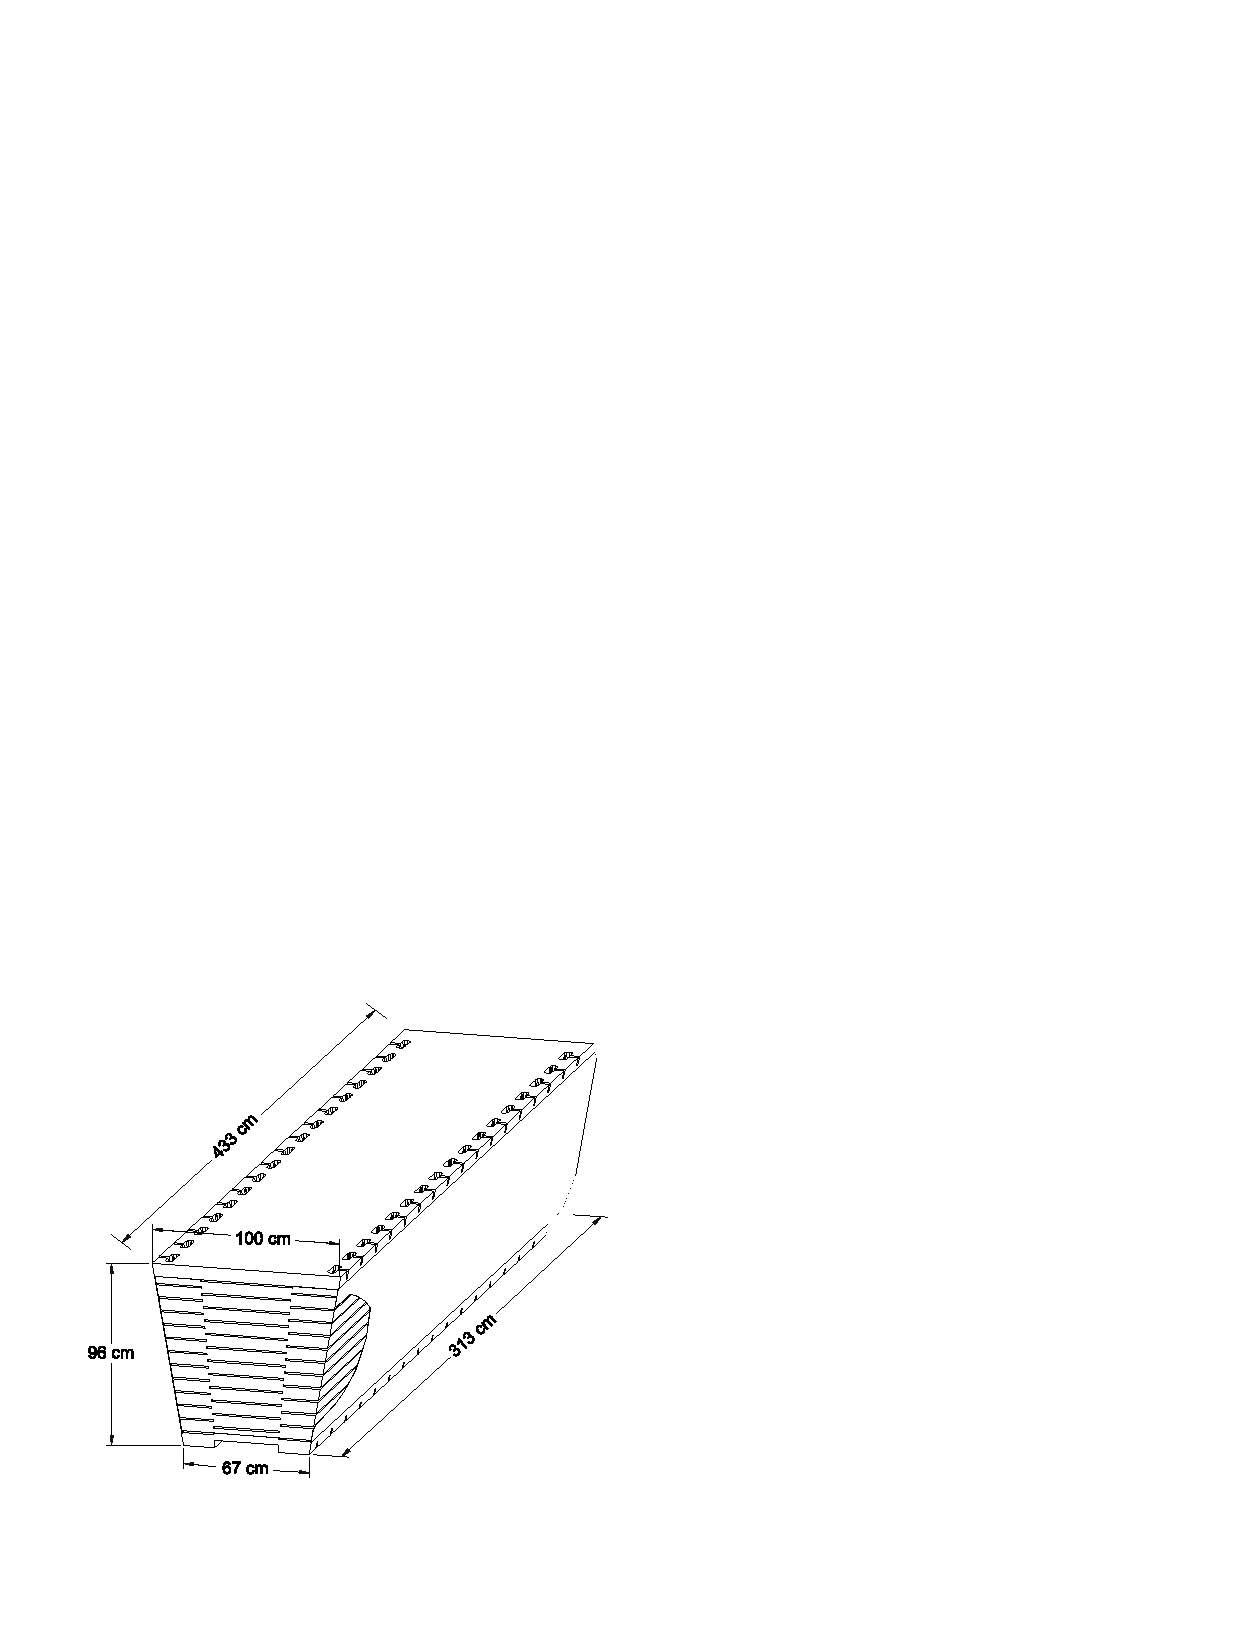
\includegraphics[width=.45\textwidth]{figures/hcal_wedge.pdf}
      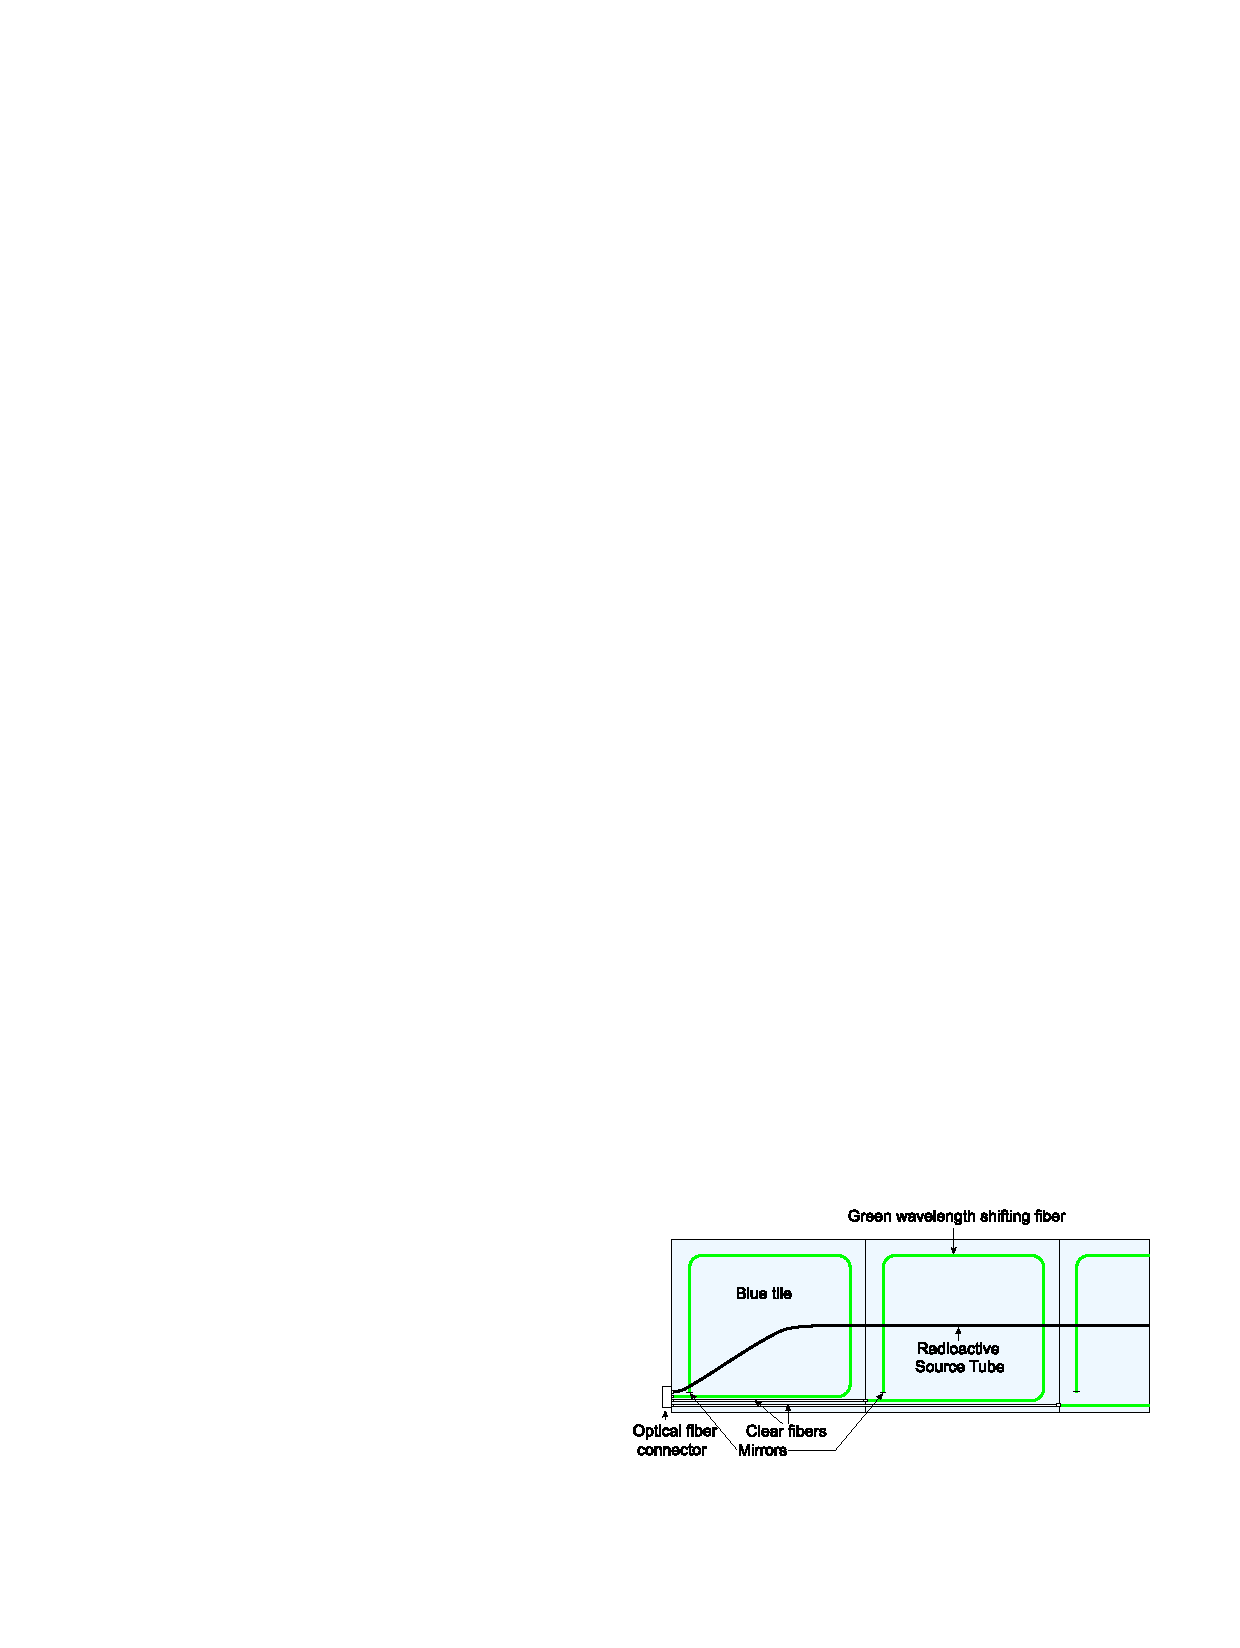
\includegraphics[width=.45\textwidth]{figures/hcal_scintillator.pdf}
      \caption{Shown on the left, a wedge of the HCAL in the barrel. The interior of the wedge is brass, and the shown slots have the scintillator modules (shown to the right) inserted so that secondary particles made in interactions with the brass will pass through them and have their energy measured. To the right, a scintillator module is shown, when a charged particle passes through the scintillator, light is generated and collected by the wavelength shifting fiber shown in green. When scintillation light is collected by the fiber, it releases green light that travels down to the clear fiber via total internal reflection and sent to be collected by photo sensors. Taken from \cite{cms_hcal_wedge}.}
      \label{fig:hcal_wedge}
    \end{figure}

    Figure \ref{fig:hcal_wedge} shows the general design of an HCAL wedge in the barrel region. Layers of brass are interspersed with scintillator strips that read out the energy of secondary particles created in the hadronic interaction. In terms of nuclear interaction lengths, the HCAL goes from about 5 nuclear interaction lengths at $\eta = 0$ up to about 10 at $\eta \ge 1.3$. Due to the shallow depth in the barrel, an outer layer of scintillator is added outside the magnet, essentially using the magnet as an absorber layer. This outer layer is called the HO and runs in the range $\eta \in [0, 1.3]$. Figure \ref{fig:hcal_layout} shows a cross-section of the HCAL including the HB, HE, and HO. With the HO in place, the minimum number of interaction lengths across the HCAL is increased to almost 12 except in the transition region between the endcap and barrel.\cite[pg. 138]{cms_jinst}

    \begin{figure}[h!]
      \centering
      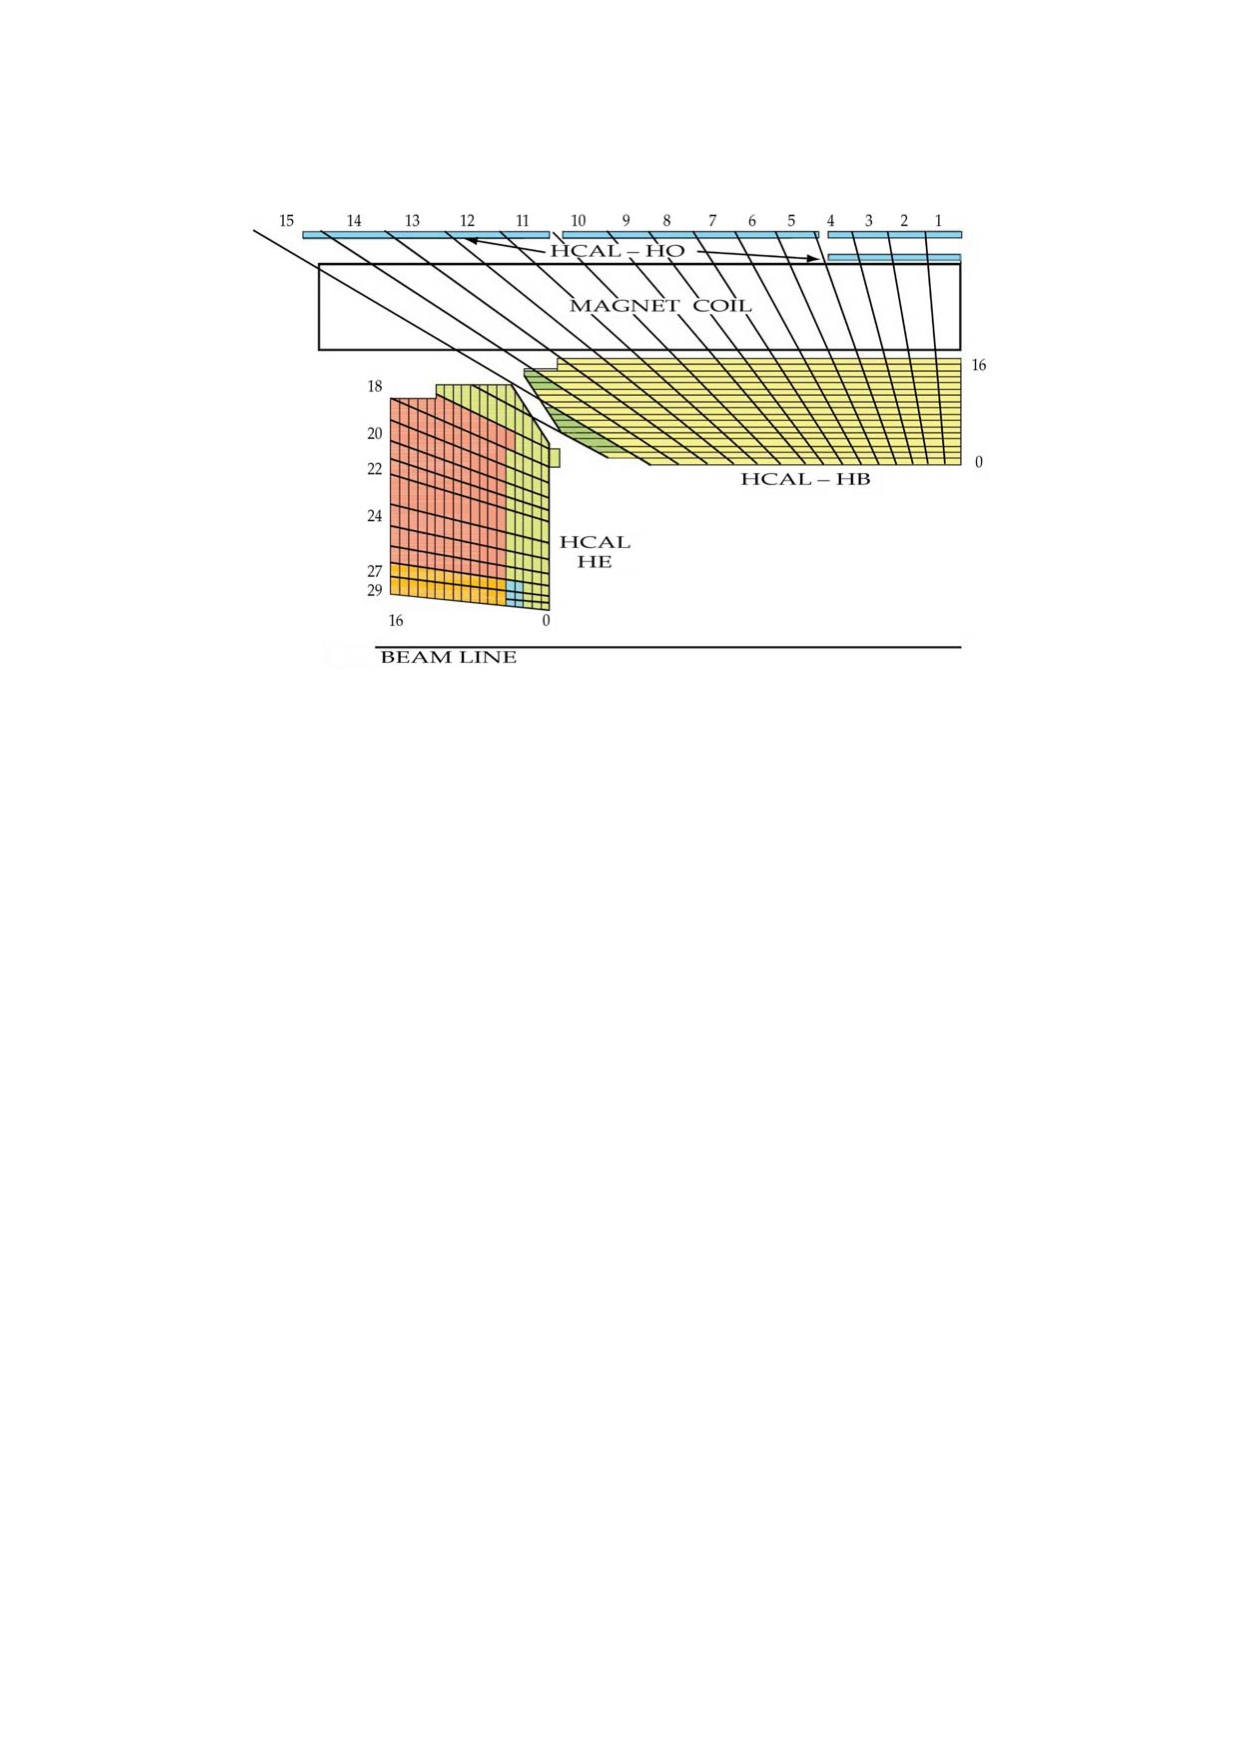
\includegraphics[width=.9\textwidth]{figures/cms_hcal_layout.pdf}
      \caption{The a cross-sectional view of the CMS hadronic calorimeter. Taken from \cite{cms_jinst}.}
      \label{fig:hcal_layout}
    \end{figure}

    Sampling calorimeters again work on the principle of scintillation, however, HCALs are meant to measure energy from neutral particles as well as charged hadrons. The strategy used in sampling calorimeters is to place dense material with many nuclei in front of the incident particles. Hadronic interactions are much more complicated than the photon and electron interactions in the ECAL because the initial state particles can vary, but in general the expected product of inelastic collisions are charged pions, which create electromagnetic cascades, and neutral particles like the $\eta$ and $\pi^0$ which quickly decay to photons. \cite[sec 35.9.2]{PDG} \cite{green_detectors} Neutron capture can also occur which makes photons that are typically out of the electronics detection capability.\todo{This is so confusing, how the hell can you say you get almost always pions for any hadronic particle?} The hadronic cascade of particles then leads into the scintillating material where scintillation light is generated and collected. Again, the amount of light collected is proportional to the energy of the charged particle \todo{why? also is the light from the $\eta$ and $\pi^0$ absorbable by the WSF?}.

    In the CMS HCAL, the absorber layers are made of brass, and the scintillator material is a proprietary plastic material, Kuraray SCSN81\footnote{excluding the very first layer where the absorber metal is stainless steel and the plastic scintillator is Bicron BC408. The very last layer also has stainless steel as the absorber metal.}. The HCAL is broken into three physical sections: the barrel (HB) extending to $\abs{\eta} \le 1.4$, the slightly overlapping endcap (HE) extending between $\abs{\eta} \in (1.3,3)$, and the slightly overlapping forward detector (HF) covering the range $\abs{\eta} \in (2.9,5)$. In this analysis, we do not use jets with energy measurements from the forward detector, that is we veto jets with $\eta > 3$.


  \subsection{The Muon System}
    The outer-most detection subsystem on CMS are the muon chamber. Muons literally put the ``M" in CMS, they are an extremely important particle for LHC physics for several reasons. \cite[sec 1.2]{muon_tdr}

    \begin{enumerate}
     \item Their production is associated with the electroweak sector, which includes the Higgs boson.
     \item They have a long enough lifetime that they can make it through the entire detector, making them easily identifiable and allowing for good momentum resolution due to their long track.
     \item Their radiative losses in the tracking system and ECAL are much smaller than electrons due to their heavier mass. They also don't deposit much energy in the HCAL because they don't interact via the strong force.
    \end{enumerate}

    The muon system on CMS is made up of three different types of detectors, all based on gas ionization.
    \begin{enumerate}
     \bitem{Drift Tubes (DTs)} Layered thin tubes with conducting cathode walls and a anode wire which runs centrally through the length of the tube. The tube is filled with Argon and CO$_2$ gas. A drift tube is shown to the left in figure \ref{fig:muon_detectors}, the length of the tube is not shown. Due to the extent in one direction, drift tubes can not give spacial resolution in all three dimensions. A typical module of these tubes has 3 layers, oriented such that the middle layer runs perpendicular to the outer layers in order to reconstruct all the position in all three dimensions. 
     \bitem{Cathode Strip Chambers (CSCs)} Six layers of anode wire planes interleaved with seven layers of cathode strips, arrayed in a cross-hatch pattern filled with gas. This configuration allows for all three dimensions of the muon's position to be reconstructed from a single module by cross referencing the voltage spikes in the strips against the voltage spikes in the wires. A schematic view of this type of detector is shown to the right in figure \ref{fig:muon_detectors}.
     \bitem{Resistive Plate Chambers (RPCs)} Parallel plate capacitors made of insulating material and filled with gas. When a muon passes through the RPC, the gas is ionized and an electron shower is generated which passes through the capacitor plates and is collected by a set of strips outside the capacitor. These detectors are interspersed throughout the entire system and mostly used to help with triggering as the response time and refractory period of these detectors are very fast compared to the 25 ns bunch crossing time. 
    \end{enumerate}

      \begin{figure}[h!]
        \centering
        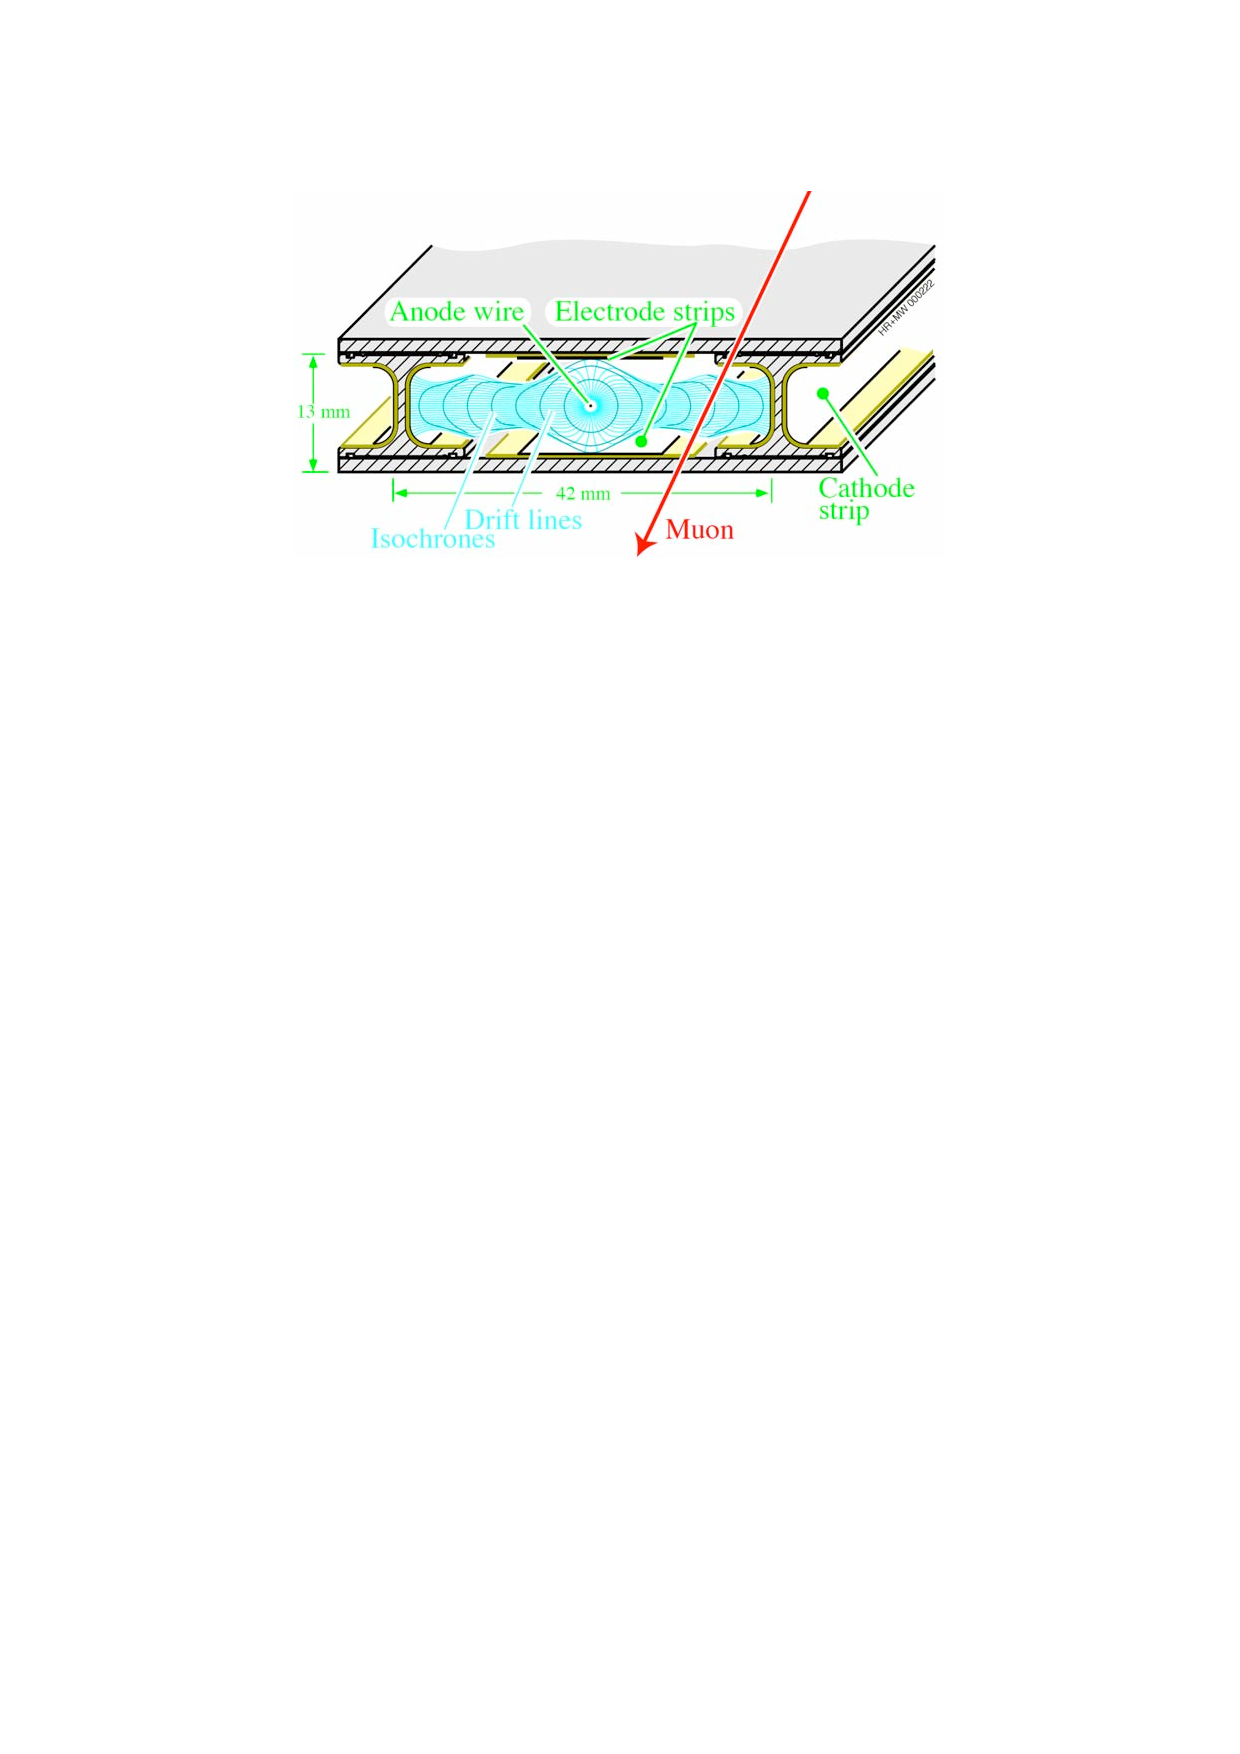
\includegraphics[width=.45\textwidth]{figures/cms_drifttube.pdf}
        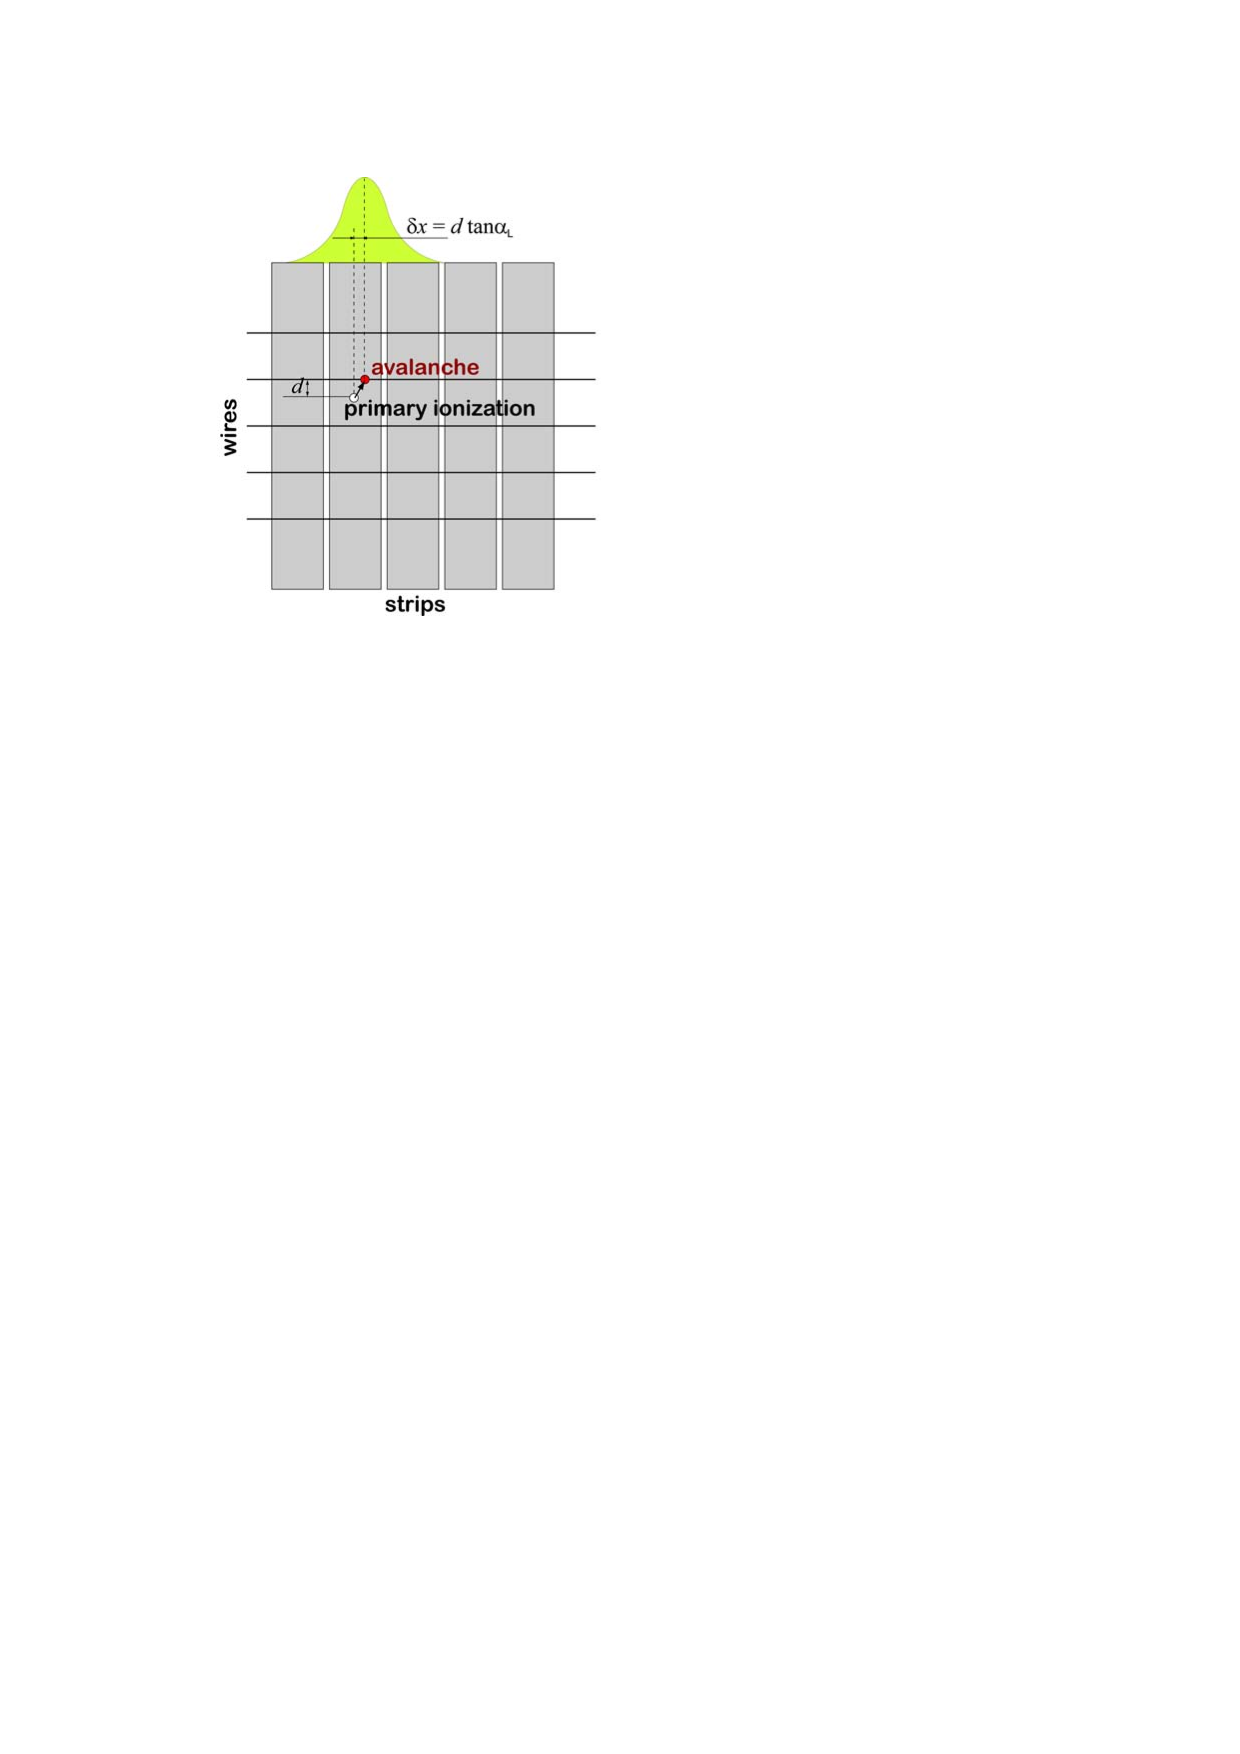
\includegraphics[width=.45\textwidth]{figures/cms_CSC.pdf}
        \caption{\textbf{Left:} A cross sectional head on view of a CMS drift tube, the tube is much longer in the omitted direction than is shown. A hypothetical path for a muon is drawn, the particle would ionize the gas in the chamber and create a spike in the potential difference between the anode and cathode as free electrons and charged ions are collected.
        \textbf{Right:} A top down view of a CSC module. A hypothetical muon hit is shown at the spot labeled ``primary ionization". A CSC module has the ability to reconstruct all three dimensions of the muon's position by cross referencing which strips collected ions and which wires collected free electrons.Taken from \cite{cms_jinst}.}
        \label{fig:muon_detectors}
      \end{figure}

      Figure \ref{fig:muon_system} shows the general layout of the muon system. In the barrel region, approximately $\abs{\eta} < 1.2$, the muon system is made up of drift tubes interleaved with RPCs. In the endcap region, approximately $\abs{\eta} \in (1.2,2.4)$, the drift tubes are replaces by CSC modules due to the higher magnetic field in this region.

    \begin{figure}[h!]
      \centering
      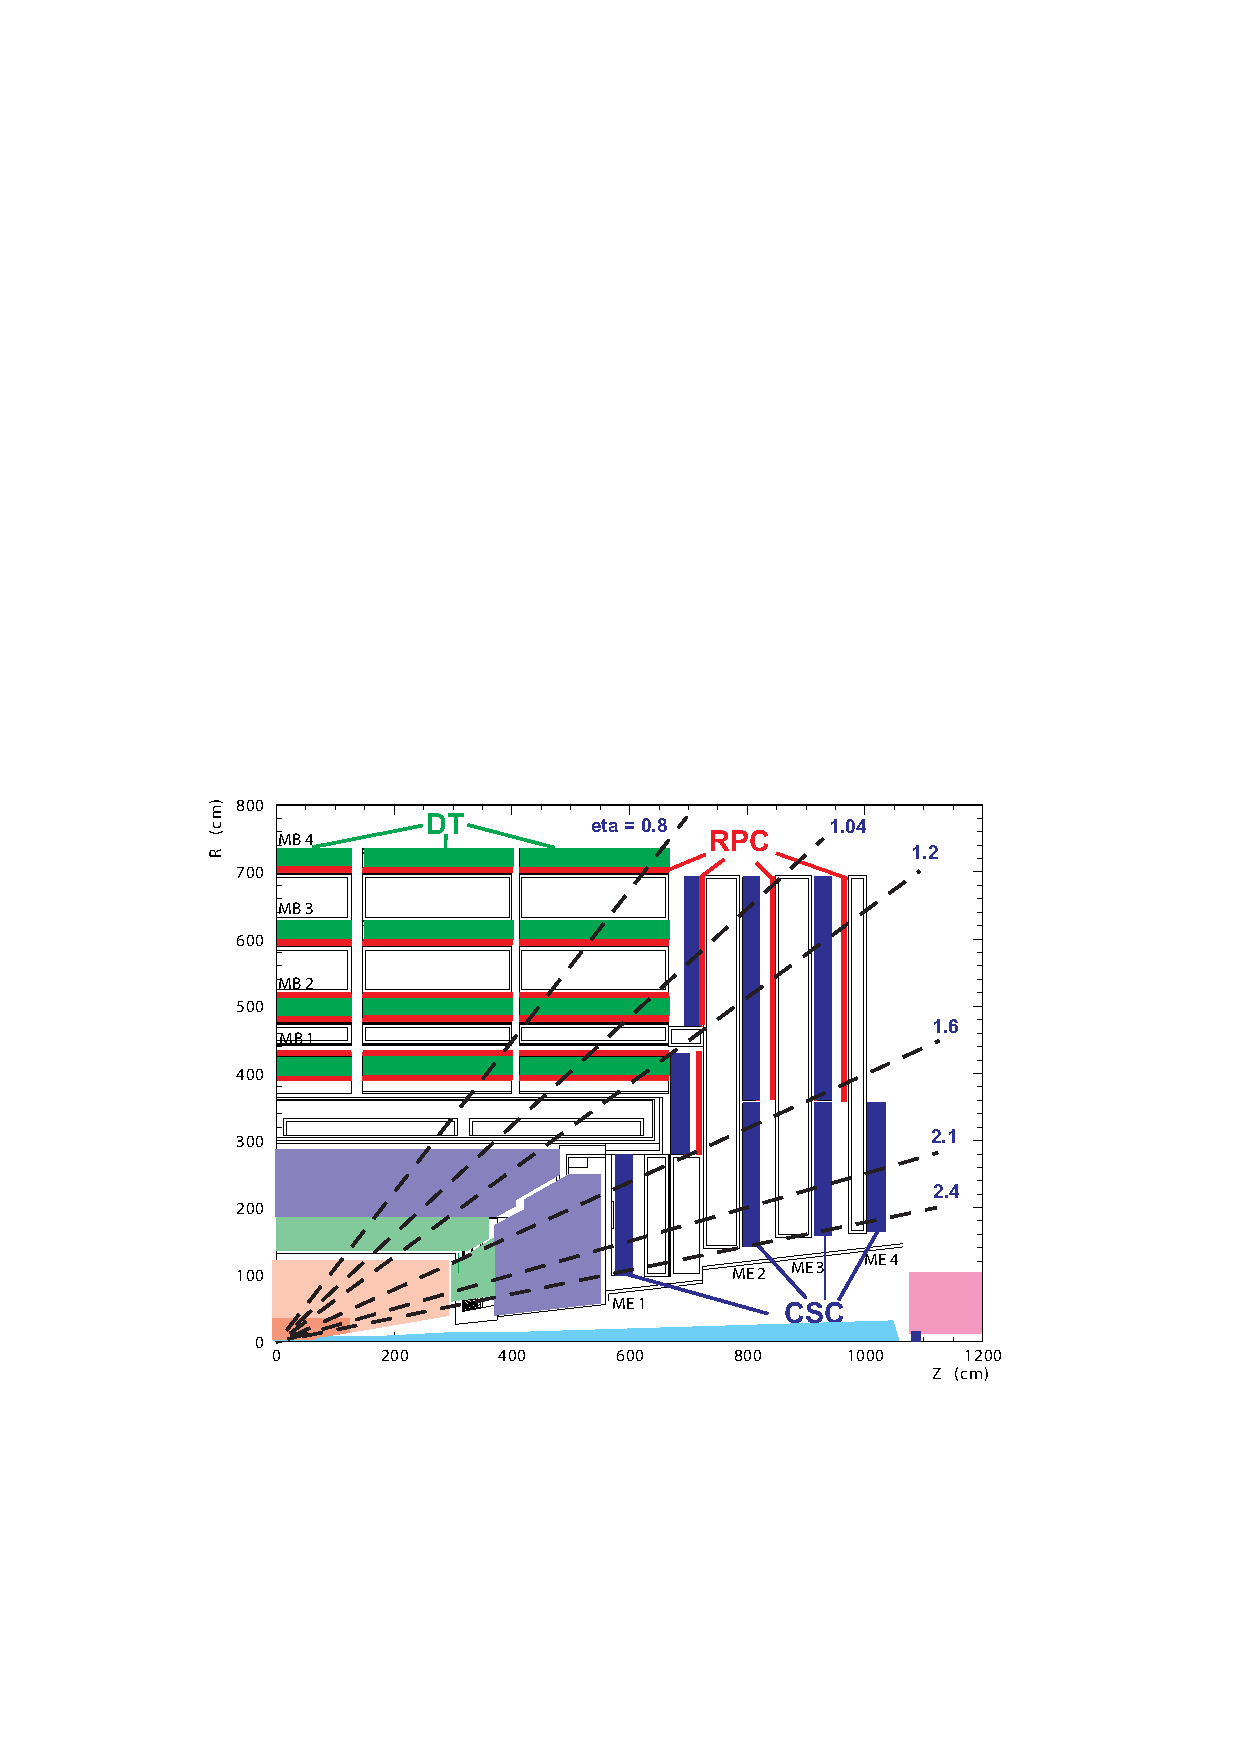
\includegraphics[width=.9\textwidth]{figures/muon_system.pdf}
      \caption{A cross-sectional view of the CMS muon system. In the barrel, with $\abs{\eta}<1.2$, drift tubes (DTs) and resistive plate chambers (RPCs) are used. In the end cap, $\abs{\eta} \in (1.2,2.4)$, RPCs and cathode strip chambers (CSCs) are used. Taken from \cite{cms_tdr}.}
      \label{fig:muon_system}
    \end{figure}

  \subsection{Event Triggering} \label{sec:event_triggering}
    A raw CMS event takes roughly 1 MB of disk space, given the rate at which bunches are crossed, storing the output from every bunch crossing would require reading out, analyzing, and storing upwards of 40 TB of data per second.\cite{trigger_tdr} The final event readout rate of the CMS detector is designed to be closer to 400 Hz, corresponding to roughly 400 MB of data per second, with the main bottleneck being offline data storage capacity and processing speed.

    In order to reduce the event rate from 40 MHz down to 400 Hz, the CMS detector employs a two-stage trigger system. The first stage, called the level 1 or L1 trigger, takes the rate down to approximately 100 kHz, a process done in hardware using application specific integrated circuits (ASICs) and field programmable gate arrays (FPGAs) for maximum speed. Events selected by the L1 system are then passed to the high level trigger system (HLT) which reconstructs physics objects in software and makes a better determination as to whether the event should be written to disk. The HLT system brings the event rate down to 100s of Hz.

    From the point of view of the L1 system, electrons and photons are identical. Decisions at level 1 for electrons and photons are made by the e/$\gamma$ L1 trigger, which mainly looks for large isolated ECAL energy deposits without a corresponding HCAL deposit. For the muon triggers, information from CSCs, DTs, and RPCs are used. Built in electronics on the detector perform track finding algorithms on hits in the DTs and CSCs independently. ``Track primitives" are created by special track finding hardware newly added for 2016. The track primitives are matched with timing and hit data from the RPCs to make decisions about muon quality and energy at L1. The processed information is sent to the global trigger system to make the final decision as to whether the event will be sent to the HLT farm.

    The HLT system consists of a processing farm with approximately 13,000 CPUs. The turn around rate for event classification is on the order of 100 ms per event. The machines in the HLT perform object identification and energy reconstruction in a way that matches the offline software suite as much as possible, though there are some optimizations made that introduce small differences to accommodate event processing at the 100 kHz rate. The HLT system is organized around the concept of ``trigger paths", which are algorithms that run object reconstruction and makes selections on these objects. A trigger path will evaluate to either true or false on an event by event basis. 

    The full list of CMS HLT trigger paths used in this analysis is presented in table \ref{table:triggers}. 

    \begin{table}[htb]
      \begin{center}
      \caption{\label{table:triggers} List of all triggers used in this analysis. }
        \begin{tabular}{l}
          \hline
          \hline
          trigger name       \\
          \hline
          di-muon triggers \\
          \hline
          --\verb=HLT_Mu17_TrkIsoVVL_Mu8_TrkIsoVVL_v*=                \\
          --\verb=HLT_Mu17_TrkIsoVVL_Mu8_TrkIsoVVL_DZ_v*=                \\
          --\verb=HLT_Mu17_TrkIsoVVL_TkMu8_TrkIsoVVL_v*=              \\
          --\verb=HLT_Mu17_TrkIsoVVL_TkMu8_TrkIsoVVL_DZ_v*=              \\
          %--\verb=HLT_TkMu17_TrkIsoVVL_TkMu8_TrkIsoVVL_DZ_v*=              \\
          --\verb=HLT_Mu27_TkMu8_v*=                                  \\
          --\verb=HLT_Mu30_TkMu11_v*=                                  \\
          %--\verb=HLT_Mu40_TkMu11_v*=                                  \\
          \hline
          di-electron triggers \\
          \hline
          --\verb=HLT_Ele17_Ele12_CaloIdL_TrackIdL_IsoVL_DZ_v*=       \\
          --\verb=HLT_Ele23_Ele12_CaloIdL_TrackIdL_IsoVL_DZ_v*=       \\
          --\verb=HLT_DoubleEle33_CaloIdL_GsfTrkIdVL_v*=           \\
          --\verb=HLT_DoubleEle33_CaloIdL_GsfTrkIdVL_MW_v*=           \\
          \hline
          e$\mu$ triggers \\
          \hline
          --\verb=HLT_Mu17_TrkIsoVVL_Ele12_CaloIdL_TrackIdL_IsoVL_v*= \\
          --\verb=HLT_Mu23_TrkIsoVVL_Ele8_CaloIdL_TrackIdL_IsoVL_v*= \\
          --\verb=HLT_Mu23_TrkIsoVVL_Ele12_CaloIdL_TrackIdL_IsoVL_v*= \\
          --\verb=HLT_Mu23_TrkIsoVVL_Ele8_CaloIdL_TrackIdL_IsoVL_DZ_v*= \\
          --\verb=HLT_Mu23_TrkIsoVVL_Ele12_CaloIdL_TrackIdL_IsoVL_DZ_v*= \\
          --\verb=HLT_Mu8_TrkIsoVVL_Ele17_CaloIdL_TrackIdL_IsoVL_v*=  \\
          --\verb=HLT_Mu8_TrkIsoVVL_Ele23_CaloIdL_TrackIdL_IsoVL_v*=  \\
          --\verb=HLT_Mu8_TrkIsoVVL_Ele23_CaloIdL_TrackIdL_IsoVL_DZ_v*=  \\
          %--\verb=HLT_Mu12_TrkIsoVVL_Ele23_CaloIdL_TrackIdL_IsoVL_v*=  \\
          %--\verb=HLT_Mu12_TrkIsoVVL_Ele23_CaloIdL_TrackIdL_IsoVL_DZ_v*=  \\
          --\verb=HLT_Mu30_Ele30_CaloIdL_GsfTrkIdVL_v*=               \\
          --\verb=HLT_Mu33_Ele33_CaloIdL_GsfTrkIdVL_v*=               \\
          \hline
          single-$\gamma$ triggers \\
          \hline
          --\verb=HLT_Photon22_R9Id90_HE10_IsoM_v*=  \\ 
          --\verb=HLT_Photon30_R9Id90_HE10_IsoM_v*=  \\
          --\verb=HLT_Photon36_R9Id90_HE10_IsoM_v*=  \\
          --\verb=HLT_Photon50_R9Id90_HE10_IsoM_v*=  \\
          --\verb=HLT_Photon75_R9Id90_HE10_IsoM_v*=  \\
          --\verb=HLT_Photon90_R9Id90_HE10_IsoM_v*=  \\
          --\verb=HLT_Photon120_R9Id90_HE10_IsoM_v*= \\
          --\verb=HLT_Photon165_R9Id90_HE10_IsoM_v*= \\
          --\verb=HLT_Photon165_HE10_v*=             \\
          \hline
          single-$\mu$ triggers \\
          \hline
          --\verb=HLT_IsoMu24_v*=  \\ 
          --\verb=HLT_IsoTkMu24_v*=  \\ 
          \hline
          \hline
        \end{tabular}
      \end{center}
    \end{table}

    The high level triggers are generally based on isolation and transverse momentum criteria. For instance, the trigger HLT\_Mu17\_TrkIsoVVL\_Mu8\_TrkIsoVVL\_DZ\_v* roughly requires that the event have at least one muon above 17 GeV of \pt and another above 8 GeV. The tags TrkIsoVVL refer to isolation requirements on the muon and DZ refers to a requirement that when their tracks terminate close to one another in the z (beamline) direction traced back to the beamline. The v* at the end of these triggers denotes that we use the latest version of the software that implements the trigger. \todo{if I get more info on the trigger tags, I'll add it here.}

    \subsubsection{Trigger efficiencies} \label{sec:trigger_efficiencies}
    Due to the low precision in the energy measurements at level 1, and the slight differences in reconstruction at the HLT and offline level \todo{is this right?}, objects near the \pt thresholds of the high level trigger do not always cause the event to be stored, we say that the triggers are not 100\% efficient. In other words, sometimes an event with an electron that is reconstructed to have 17 GeV of \pt offline will not pass the Ele17 trigger because it was either not selected at level 1, or it was reconstructed to have less \pt than 17 GeV by the HLT reconstruction software.

    The rate at which this occurs can be treated statistically. It is mainly a function of the offline reconstructed \pt because all of the triggers used in this analysis are based on the \pt of some object. As an example, figure \ref{fig:mu_l1_eff} shows the L1 trigger efficiency for the single muon L1 25 GeV trigger in the 2017 dataset\footnote{this analysis uses the 2016 dataset, the figure is only for illustration} at the \pt threshold of 25 GeV (the target threshold for the single muon trigger). As can be seen in the figure, muons with \pt $\le 8$ GeV (as reconstructed offline) are almost never selected by the 25 GeV L1 trigger. The trigger never selects 100\% of the muons, even at very high energies. However, after about 30 GeV, the percentage of muons selected plateaus. We say that the trigger is \emph{fully efficient} at 30 GeV to denote this feature, which is common to all trigger turn-on curves.

    \begin{figure}[h!]
      \centering
      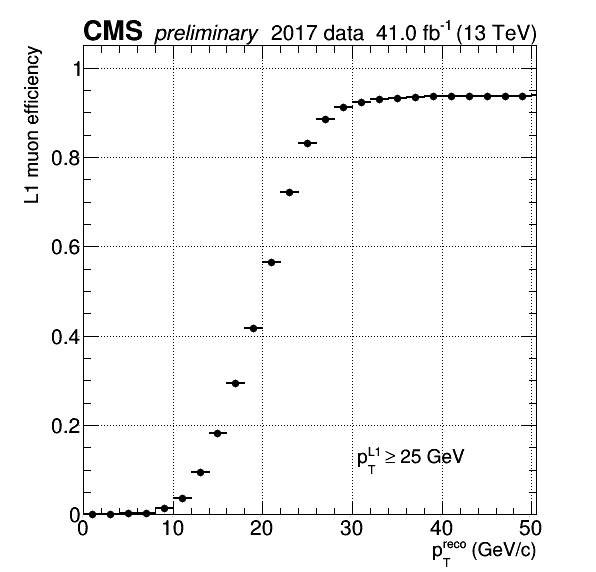
\includegraphics[width=.7\textwidth]{figures/muon_l1_eff.png}
      \caption{The trigger efficiency for the L1 muon 25 GeV trigger. The system attempts to pass all muons with 25 GeV of \pt to the HLT system, though the fast calculation with on-board hardware at L1 does not capture all muons at this threshold. The plot is made by selecting events with two muons reconstructed offline where the leading \pt muon has \pt above 27 GeV and has passed the L1 25 GeV trigger. The second muon is then checked to see whether it also passed the L1 criteria. This method is called tag-and-probe. As can be seen, the trigger is never at 100\% efficiency, but a plateau exists around 30 GeV where we call the trigger \emph{fully efficient}. Taken from \cite{mu_l1_twiki}.}
      \label{fig:mu_l1_eff}
    \end{figure}

    Trigger efficiencies enter this analysis in two places. First, MC used in this analysis has the trigger efficiencies built in, that is MC events are tagged as passing for failing triggers at rates equal to the trigger efficiencies. Second, the difference in the efficiencies for the electron and muon trigger paths in this analysis are part of what is corrected by the \rsfof factor, which will be described in section \ref{sec:rsfof}. In short, this analysis uses the symmetry between production rates of electrons and muons in certain physics processes to make certain background predictions. That symmetry is broken by the fact that, along with different offline ID requirements, the trigger efficiencies for electrons and muons at the same \pt will, in all likelihood, not be identical.

\section{Physics Objects}
  After energy deposits are read out from the detector they are used to reconstruct \emph{physics objects} that can then be further analyzed to discover new particles and interactions. The layout of the CMS detector was chosen carefully to allow for the identification of several groups of particles:

  \begin{enumerate}
    \bitem{Jets} sprays of particles containing mostly hadrons and photons. An ideal jet will leave multiple tracks in the tracker that point back to the same spot on the beamline and deposit a large amount of energy in the HCAL and a smaller amount of energy in the ECAL as well.
    \bitem{Isolated Photons} single photons that were likely produced in the hard collision, rather than being radiated by a charged particle in the detector. An ideal single photon will leave no tracks and deposit energy in only the ECAL
    \bitem{Isolated Electrons} single electrons that were likely produced in the hard collision, rather than being produced as a secondary particle in the detector (for instance in pair production). An ideal isolated electron will leave a hit in every layer of the tracker and deposit energy only in the ECAL along the line traced out by the tracker hits. Bremsstrahlung photons are typically radiated from electrons in the tracker, therefore we should also expect kinks in electron tracks accompanied by energy deposits in the ECAL associated with the kinks.
    \bitem{Muons} expected to leave hits in every layer of the inner tracker. When extrapolated through the detector, the inner tracker hits should match up with standalone muon tracks in muon system. Nearly no energy should be deposited in the ECAL or HCAL
    \bitem{Tagged Jets} jets that have been tagged as originating from a specific particle, for instance a b-quark or a $\tau$-lepton. These objects typically use information from the jet tracks to give a measure of how likely a specific jet was to represent the decay dynamics of the specific particle in question.
  \end{enumerate}

  In order to reconstruct these objects from energy deposits in the detector, CMS employs an algorithm called particle flow\cite{cms_particleflow} which will be outlined in section \ref{sec:particle_flow}. However, the first step in object generation is the vertex and track reconstruction.

  \subsection{Track Reconstruction} \label{sec:track_reconstruction}
    Track reconstruction is the process of turning hits in the tracker into proposed trajectories for charged particles. The track finding software used by CMS is called the Combinatorial Track Finder \cite[pg. 12]{cms_track_vertex}, which is based off of the Kalman filter \cite{kalman_filter} track fitting method. The basic idea is to work iteratively, first building the more ``obvious" tracks for high \pt particles, and then removing their hits from the collection thus making the next track easier to find.

    Each iteration begins with a ``seed track." In the first iteration, the seed tracks are built from collections of 3 hits, one in each layer of the pixel tracker, with curvature tolerance such that the particle \pt is larger than 0.8 GeV. In later iterations, seed tracks are built from hit groups that are missing a layer in the pixel tracker, or even from hit groups solely in the strip tracker to accommodate the possibility of secondary decays.

    The seed tracks are extrapolated into the next layer of the tracker, taking into account the uncertainty in the track's position and momentum, by assuming a constant magnetic field and disregarding the possibility of multiple scattering and energy loss when the particle is not within a tracker layer\footnote{Energy loss is modeled statistically when the particle is in the tracker material, which has the effect of broadening the track uncertainty.}. After the expected trajectory is built, hits within some number of standard deviations of the expected trajectory in the nearest tracker layer are collected into groups of possible energy deposits for the particle\cite{track_uncertainty}. This process can include the possibility of adding a ``ghost hit" if no hit was found in a module along a particular possible trajectory. 

    A $\chi^2$ test is then performed between the expected trajectory and the hit groups, taking into account the hit and trajectory uncertainties. The number of hits in a typical event is enough that most seed trajectories can be associated with multiple paths at each layer. After possible trajectories are built out of the hit groups, only a small number of possible trajectories are extrapolated into the next layer based on their $\chi^2$ values and number of ghost hits. This process is repeated until track quality parameters, for instance too many ghost hits, can no longer be satisfied at the next layer. After the hits in the detector are organized into tracks, another fit is applied to smooth the track trajectory using a Kalman filter fit. During this stage, hits which are outliers can be disassociated with the trajectory and added back the general collection of hits. The smoothing step occurs again until all outliers have been removed\cite[sec 4.3]{cms_track_vertex}.

  \subsection{Vertex Selection} \label{sec:vertex_selection}
    Each event recorded at CMS has a \emph{primary vertex}, which is roughly defined as the point along the beamline at which the highest energy tracks emerged. This process involves first selecting the highest quality tracks from track reconstruction, then clustering them into sets that seem to originate from roughly the same point along the beamline, and finally fitting the location of the vertex based on the cluster end-points. 

    Tracks are selected based on the impact parameter to the beamline ($<$5), number of hits ($\ge 2$ pixel, $\ge 5$ pixel+strip), and the $\chi^2$ value from the track fit ($<20$). Again the vertex selection is an iterative process, at first all tracks are assumed to come from one vertex, then at each step vertices can be split. In practice this is achieved with a process called \emph{deterministic annealing} (DA) which is based on ideas from thermodynamics of minimizing free energy at some temperature. 

    Once vertices are identified and tracks are assigned to a vertex, vertices with at least two tracks are fitted using an adaptive vertex fitter \cite{adaptive_vertex_fitter} to compute position and quality quantities such as the position of the vertex in space and weights for the likelihood that the tracks associated with the vertex genuinely began there. The weight, $w_i$, of a track $i$ is close to 1 if its position is near the vertex and close to 0 if its position is several standard deviations away. The quantity \ndof is used a quality parameter defined as

    \[
      \ndof = -3+2 \sum \limits_{i=1}^{\text{\# tracks}} w_i.
    \]

    When more than one primary vertex can be found in an event, the vertex with the highest scalar sum of \pt for all the tracks associated with the vertex is chosen. In the analysis presented in this thesis, we only select events where the primary vertex has \ndof $>4$, and the vertex is located within 24 cm from the center of the detector along the beamline direction and within 2 cm from the beamline in the transverse plane.

  \subsection{Particle flow} \label{sec:particle_flow}
    The particle flow algorithm is in charge of turning tracks and energy clusters from the calorimeters into physics objects with energy, momentum, and location information. It achieves this goal through an iterative process of linking energy deposits, much like the tracking algorithm outlined above in sec \ref{sec:track_reconstruction}. Energy deposits in the Calorimeters, tracks in the inner tracker, and tracks in the muon chambers are all linked together pairwise based on various criteria \cite[sec. 4]{cms_particleflow}. The exact criteria for particle flow identification can be found in detail in the previous citation. In broad strokes, the energy deposits in the detector are turned into electrons, photons, muons, charged hadrons, and neutral hadrons based on the following criteria:

    Electrons are identified when tracks in the inner tracker are linked with energy deposits in the ECAL. When such a link is found, a Gaussian Sum Filter (GSF) \cite{cms_gsf} algorithm reconstructs the track because kinks in electron tracks due to bremsstrahlung radiation are not handled well by the standard Kalman Filter tracking as it does not account for momentum changes due to radiation. An energy deposit in the ECAL without a corresponding track is reconstructed as a photon. Muons are reconstructed by comparing tracker muons, tracks in the inner tracker with at least one associated hit in the muon system, with standalone muons, reconstructed tracks in the muon system. Reconstruction of a muon requires a tracker muon and a standalone muon with compatible trajectories and the absence of a large energy deposit in the calorimeters. Finally, energy deposits in the HCAL are considered neutral hadrons, and tracks which leave energy deposits in the HCAL, but not the ECAL, are considered charged hadrons.

    After the energy deposits are clustered into particles, we use the anti-KT algorithm with a radius of $R=0.4$ in $(\eta, \phi)$ space to cluster particles into jets.\cite{cms_jet_performance} 


  \subsection{Electron Measurement Pipeline} \label{sec:electron_measurement_pipeline}
    High energy electrons have energy measurements based mainly on their ECAL deposit. When a charged particle moves through the tracker, a momentum measurement can be found due to its curvature. However, due to the likelihood of bremsstrahlung radiation, the sagitta of an electron track has a high chance of being malformed, containing kinks caused when a high energy photon is emitted. Since the sagitta momentum measurement assumes the free motion of a charged particle in a magnetic field with constant energy, the track from an electron that emits a high energy photon can not be used to determine the electron's original momentum.

    When the electron reaches the ECAL, almost all of its energy is deposited within a small region. For instance, a 120 GeV electron typically deposits 95\% of its energy within a 5x5 crystal array. However, when passing through the tracker, an electron will radiate 33\% of its energy an average before it reaches the ECAL, this figure inflates to about 86\% of the energy for electrons that pass through the densest parts of the detector near $\abs{\eta} = 1.4$ (seen in fig. \ref{fig:tracker_material_budget}). Due to the bending of the electron in the magnetic field, bremsstrahlung photons will tend to spread out in the $\phi$ direction, with the spread in the $\eta$ direction being mostly negligible \cite[sec. 4.1]{Electron_reco}.

    In addition to the momentum measurement, the Kalman Filter track building method is poorly suited for electron tracks as it also assumes the motion of constant energy charged particle in a magnetic field. In order to construct electron tracks, CMS also utilizes another track finding algorithm developed specifically for the reconstruction of electron tracks called the Gaussian Sum Filter (GSF)\cite{cms_gsf}, which can be roughly intuited as several Kalman Filters assuming different radiation rates running in parallel. 

    A high energy photon radiated by an electron will leave an energy deposit in the ECAL and change the trajectory curvature for the electron. These deposits can typically be found by tracing tangents from the electron's trajectory to the ECAL due to the high likelihood that bremsstrahlung photons will be emitted along the electrons momentum vector \todo{can I find a source that says how much this is true as a function of energy?}. 

    To measure the total energy of the electron, the energy of the bremsstrahlung photons should be included as well, and so the ECAL clusters energy deposits into \emph{superclusters}. Track reconstruction with the GSF algorithm is similar to that of the Kalman filter described in sec. \ref{sec:track_reconstruction}, but, in addition to seeding tracks from pixel hits, ECAL superclusters are also used as seeds and tracks leading into the end of a supercluster are extrapolated backwards towards the beamline assuming both charge hypotheses. \todo{is there consistency checking that the photons come at places where there are reasonable kinks?} Ultimately, the electron's momentum is reconstructed using a weighted combination of the track momentum and supercluster energy. Electrons with energy less than 15 GeV use almost exclusively the pixel track momentum, while electrons with energy greater than 250 GeV use the supercluster measurement exclusively. 

    A series of corrections are applied to the supercluster energy. These corrections are derived in simulation where true electron energies and momenta are known to perfect precision. They include the effect of deposited energy not being properly associated the supercluster, loss of energy due to gaps in and between detector modules, pileup, and so on.\cite[sec 4.8]{Electron_reco} 

    Differences in data and simulation are due mainly to imperfect modeling of the tracker material. Figure \ref{fig:electron_Z_resolution} shows the dilepton mass of Z$\to$ee events in both data and simulation. The events in data are estimated to have 2\% background contamination\cite[sec. 4.5.1]{ecal_energy_reco} and are selected by requiring two opposite charge electrons with dilepton mass in the range 60-120 GeV, and where each lepton has at least 25 GeV of \pt. These comparisons are made for different ranges of $\eta$ and \pt as well as instantaneous luminosity and ``quality class" based on the scale and number of bremsstrahlung photon deposits found in the electron's supercluster. Although the agreement between data and simulation is excellent, a correction is applied to data so that the overall energy scale matches that seen in simulation, and a correction is applied to simulation so that the energy resolution matches that seen in data. \todo{What does it mean for the simulation correction? Where is that propagated?}

    \begin{figure}[h!]
      \centering
      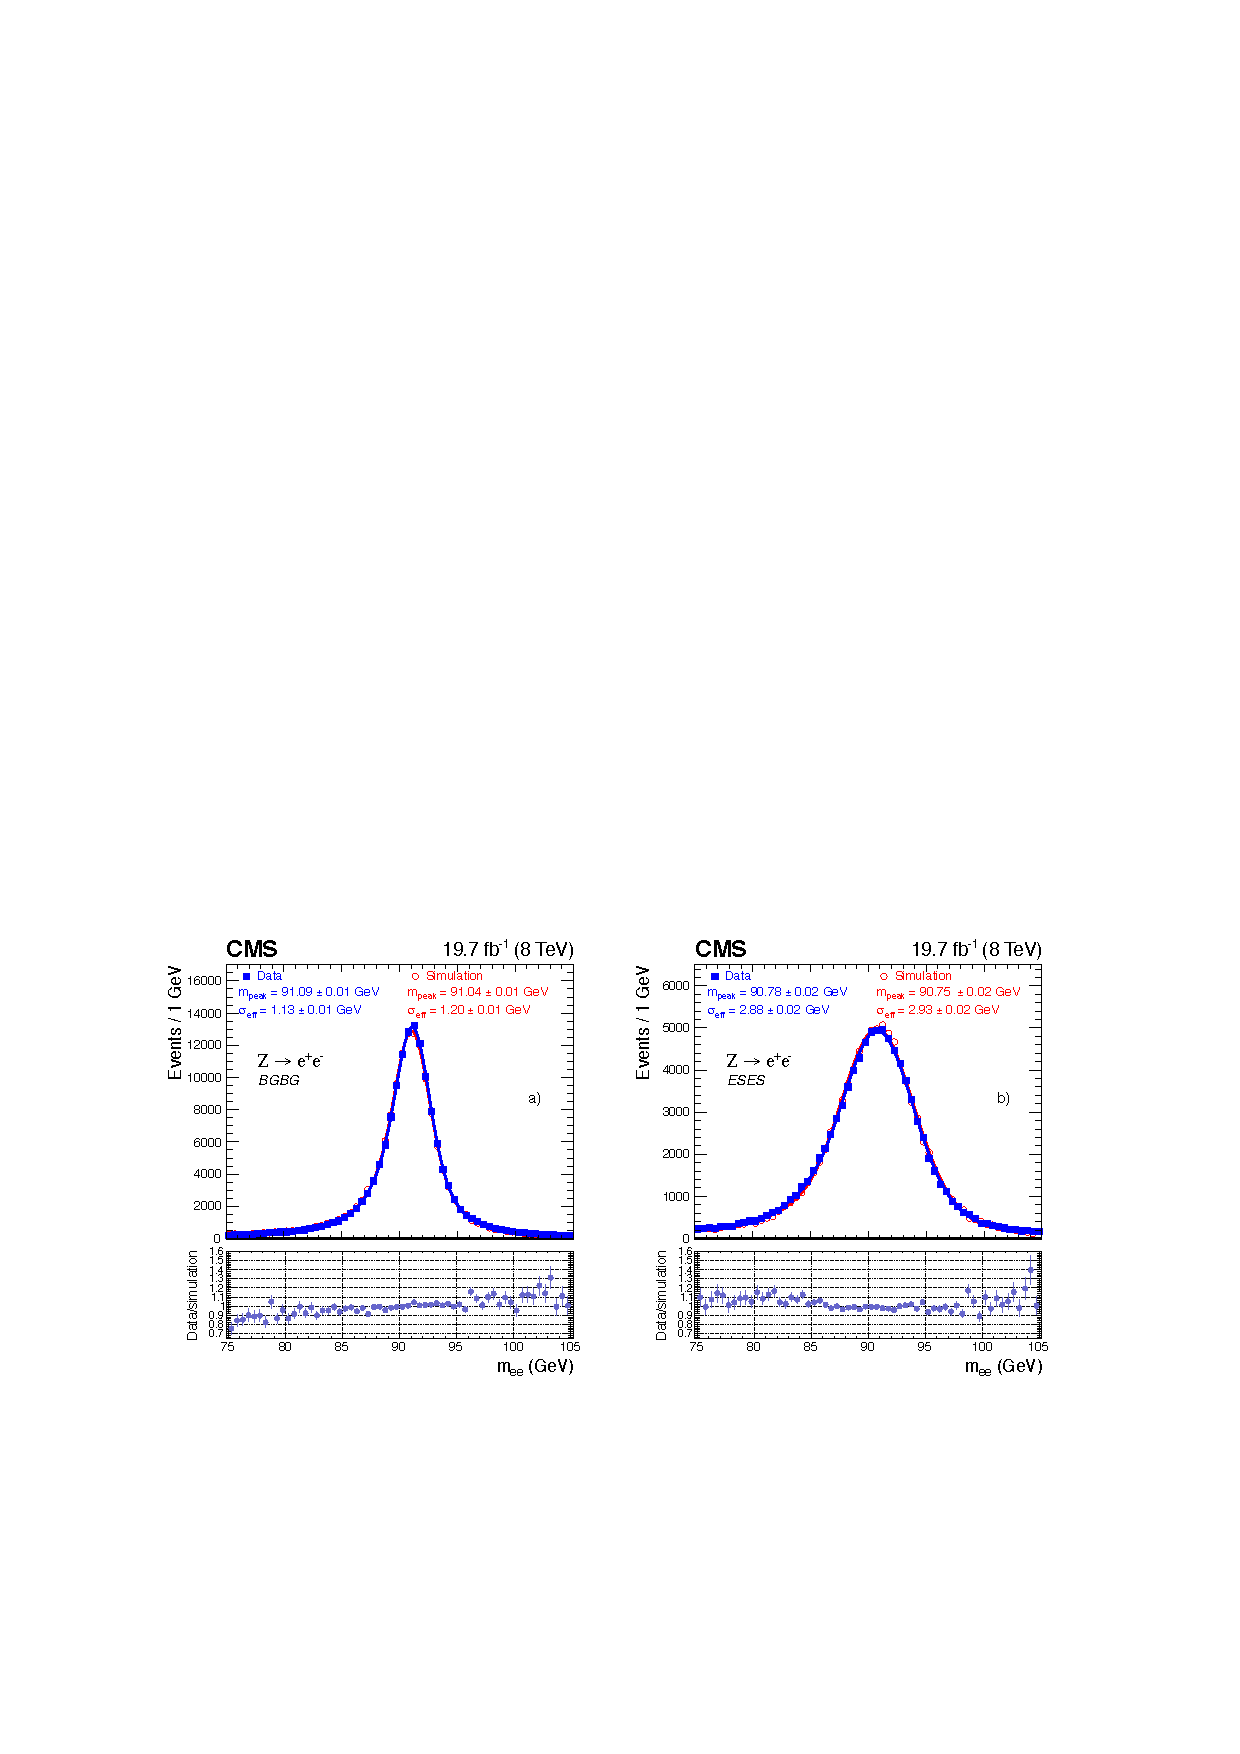
\includegraphics[width=.7\textwidth]{figures/electron_Z_resolution.pdf}
      \caption{Data and simulation of Z to di-electron events at 8 TeV. On the left, only electrons in the barrel which have not undergone any bremsstrahlung radiation are plotted, these should be the easiest class of electrons to measure. To the right, only electrons in the endcap with multiple subclusters in their ECAL supercluster are plotted, these should be the hardest class to measure. In both cases there is excellent agreement between data and simulation meaning that the corrections applied to data derived from simulation are reasonable. Additionally, the peak Z masses match the established value to approximately the percent level in both cases. Taken from \cite{Electron_reco}.}
      \label{fig:electron_Z_resolution}
    \end{figure}

  \subsection{Muon Measurement Pipeline} \label{sec:muon_measurement_pipeline}
    Muon reconstruction starts with tracks from the inner and tracker and muon system. Muon identification in particle flow can come from several sources, but in this analysis we only use ``global muons". 

    Tracks found in the muon system are called ``standalone muons." For each standalone muon track, a collection of possible tracks in the inner silicon tracker that could correspond to the standalone muon are identified. These tracks are then propagated forward to a common plane with the standalone muon track which is propigated backwards to the same plane. Position information on that plane, along with momentum measurements and uncertainties are used to select the best match. \cite[sec 3]{cms_muons} \cite[sec 5.1]{muon_reco_AN} After a match is found, the Kalman Filter track fitting method is applied from scratch to the hits in the inner tracker and muon system to smooth the overall combined track, which constitutes the global muon track used in this analysis.

    Muon momenta are computed from the sagitta of the track. At high energies, the segment of the track in the tracker provides the best momentum resolution due to the tighter density of the inner tracker modules. At energies above approximately 200 GeV, the tracks in the muon system provide a better measurement due to their longer lever arm. \todo{Is this correct?} 

    Again, a series of corrections to the muon momentum are derived using simulation. Because the measurement of the momentum is done via the track sagitta, as explained in appendix \ref{sec:sagitta}, the largest source of mismeasurements comes from misalignment of the tracker and muon modules, incorrect modeling of the magnetic field, and mis-modeling of the tracker material.\cite[sec. 6]{cms_muons} In general, the CMS detector is built to ensure that the energy resolution of muons (measured in terms of their \pt) is good to within 1\% for a 100 GeV muon and 10\% for a 1 TeV muon. In other words, CMS was built with the requirement that $\frac{\sigma(\pt)}{\pt} \approx 0.01$ for $\pt \approx 100$ GeV and $\frac{\sigma(\pt)}{\pt} \approx 0.1$ for $\pt \approx 1$ TeV. 

    Figure \ref{fig:muon_Z_resolution} shows the results of the SIDRA study that don't actually tell you anything about the energy resolution.

    \todo{Looks like this isn't what we actually get though, that figure is WAAAYAYYYYYY worse than 1\%. Why does CMS not make a fucking plot that says, here's what the Z peak is supposed to look like, here's what our fucking data says? Why? Probably because it would show that no one knows what the fuck they are doing and all of our analyses are garbage.}

    \begin{figure}[h!]
      \centering
      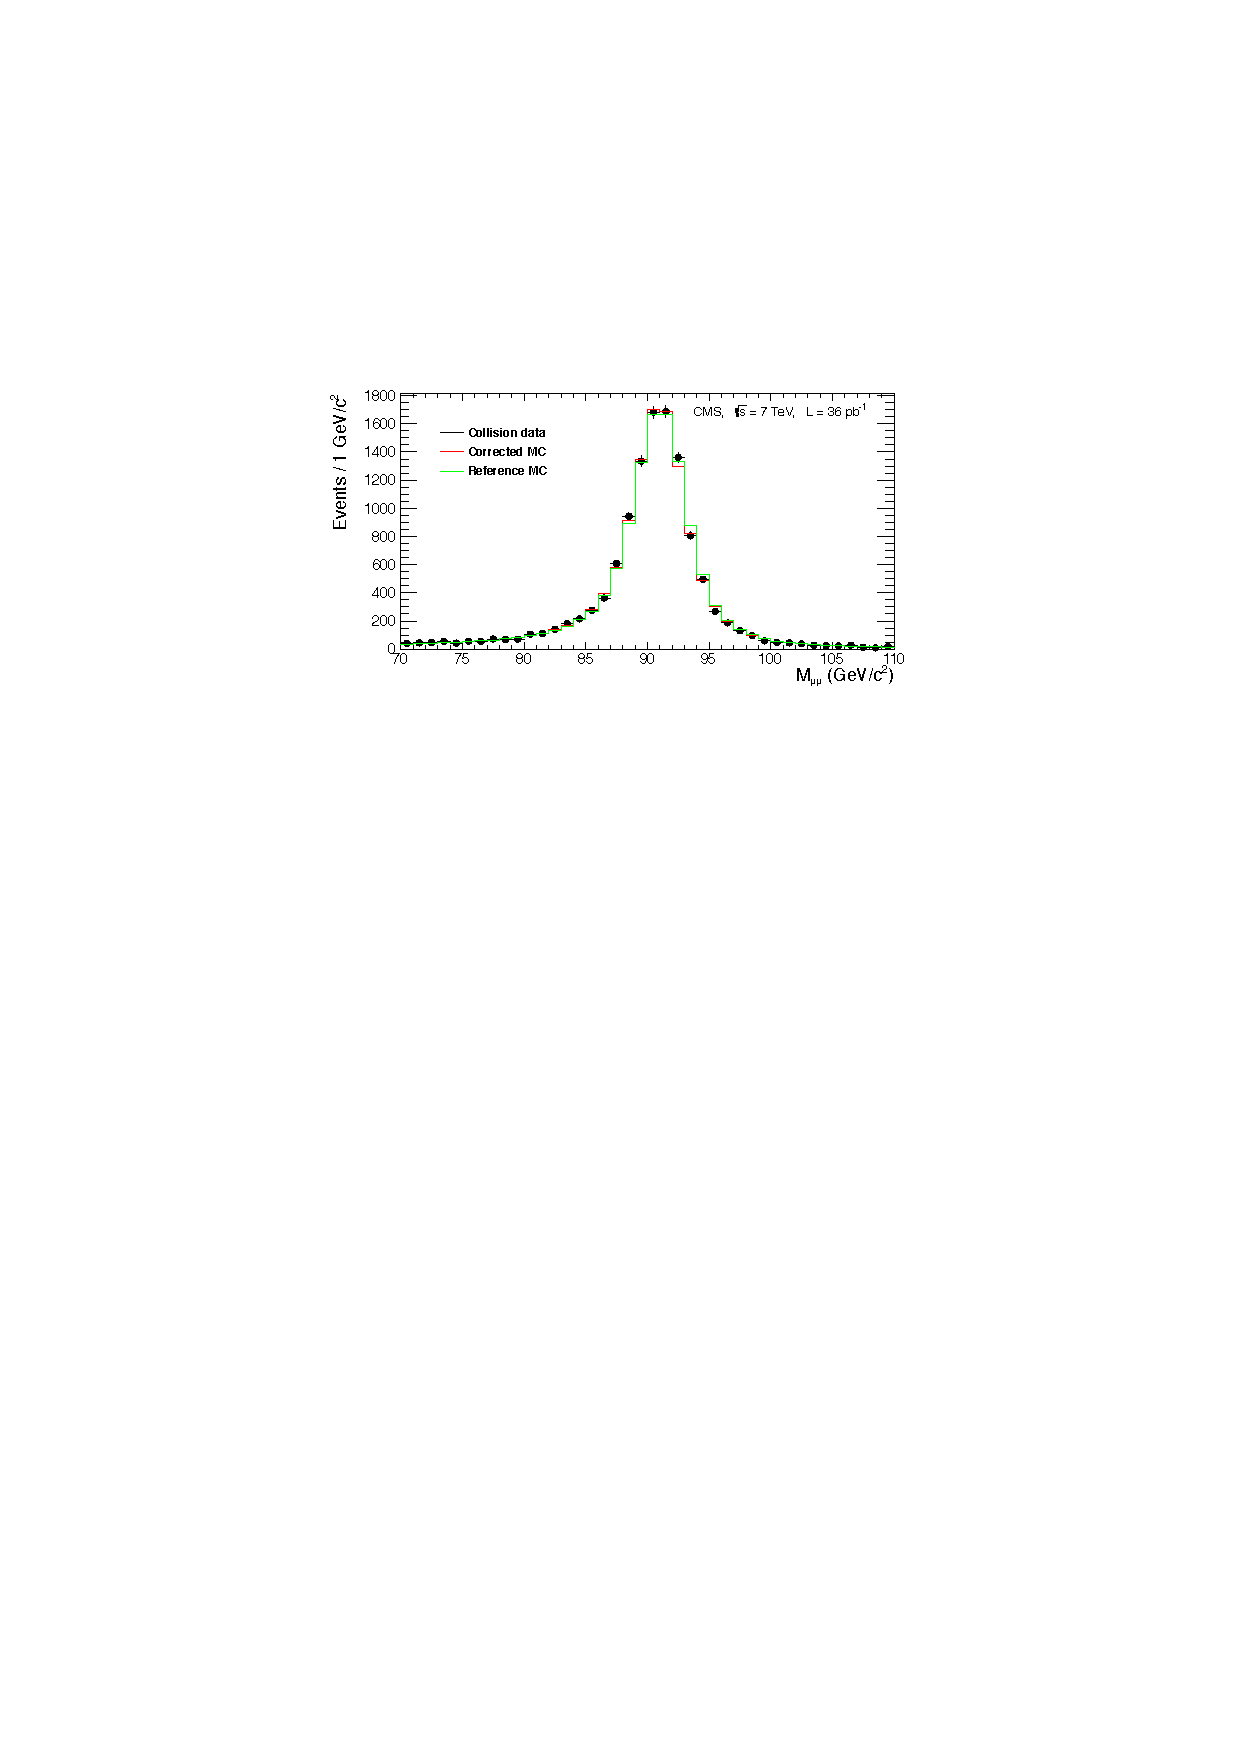
\includegraphics[width=.7\textwidth]{figures/muon_Z_resolution.pdf}
      \caption{Data and simulation of Z to di-muon events at 7 TeV. The black dots represent data from the detector, while the green line-shape represents the expected line shape for Z$\to\mu\mu$ events using the baseline detector simulation. Corrections are derived from this data and propagated forward Taken from \cite{cms_muons}.}
      \label{fig:muon_Z_resolution}
    \end{figure}
    
  \subsection{Photon Measurement Pipeline}
    ECAL measurements, lepton conversions. Photons probably pair produce in higher eta ranges, how does that work?
    \todo{plot for photon energy resolution?}
  \subsection{Jets} \label{sec:jets}
    Describe charged hadron subtraction, JECs ~\cite{JERC}, \cite{JEC_2016}
    pfCHSjets with L1FastL2L3 corrections (MC), L1FastL2L3L2L3residual corrections (data).
    \verb=Summer16_23Sep2016V3= JEC payload used to correct jets
    Need to put in blurbs about L1 Pile Up Corrections, L2L3 MC-Truth Corrections, and L2L3Residual Corrections (data only). Short descriptions here: https://twiki.cern.ch/twiki/bin/view/CMS/IntroToJEC 

    pfjetID

    Good info in Vince's Thesis and here: https://arxiv.org/pdf/1607.03663.pdf
    Roughly: L1 -- (pileup offset correction) pileup correction use QCD MC to get avg energy change to jet with and without pileup overlay. Look in 2D plane of $\eta$ and \pt, get correction.
    L2L3 -- (simulated response correction) Look at dijet events in MC, see how energy reco is different across \pt and $\eta$, correct for it.
    L2L3 Residual -- (Residual Corrections for data) Make MET 0 in dijet/ZJet/GammaJet events.

    jet energy mismeasurements are a function of the absolute scale of energy

    \todo{plot for jet energy resolution?}
  \subsection{B-Tagging} \label{sec:b-tagging}
    What is B-tagging? What do they look at? What's the false positive rate that we use?

  \subsection{MET Reconstruction} \label{sec:MET_reco}
    Make sure to add bits about sources of MET and the Type 1 correction
  \subsection{MET Filters} \label{sec:met_filters} 
    We apply certain filters that kill events, these are called MET filters but include things like beam halo as well.

\section{Monte Carlo} \label{sec:monte_carlo}
  Physics generated using Madgraph 5 interfaced with pythia8 for showering. List samples and their generator.
  SUSY models are also simulated using the madgraph package, but are then passed through the fastsim toolkit \cite{fastsim} rather than the full GEANT simulation. Statistical uncertainty in MC.
  \subsection{Summary of Simulated Samples} \label{sec:summary_of_simulated_samples}
    
    In this section we list all the Monte Carlo (MC) samples used for this analysis as well their generator and detector simulation.

    In this section we list the MC samples used for the \pt reweighting closure test.
      \begin{table}[htb]
        \begin{center}
          \scriptsize
          \caption{\label{tab:closuremc} List of MC samples used for the closure test.}
          \begin{tabular}{l|l|c}  
            \hline
            \hline
            Process & Dataset Name                                                            & Cross Section [pb]\\
            \hline
            \gjets   & \verb=/GJets_DR-0p4_HT-40To100_TuneCUETP8M1_13TeV-*-v1=                & 18560    \\
                     & \verb=/GJets_DR-0p4_HT-100To200_TuneCUETP8M1_13TeV-*-v1=               &  5000    \\
                     & \verb=/GJets_DR-0p4_HT-200To400_TuneCUETP8M1_13TeV-*-v1=               &  1079    \\
                     & \verb=/GJets_DR-0p4_HT-400To600_TuneCUETP8M1_13TeV-*-v1=               &   125.9  \\
                     & \verb=/GJets_DR-0p4_HT-600ToInf_TuneCUETP8M1_13TeV-*-v1=               &    43.36 \\
            \hline   
            \zjets   & \verb=/DYJetsToLL_M-50_TuneCUETP8M1_13TeV-*_ext1-v2=                     &  6021    \\
                     & \verb=/DYJetsToLL_M-50_HT-100to200_TuneCUETP8M1_13TeV-*_ext1-v1= &   181.3   \\
                     & \verb=/DYJetsToLL_M-50_HT-200to400_TuneCUETP8M1_13TeV-*_ext1-v1= &    50.42  \\
                     & \verb=/DYJetsToLL_M-50_HT-400to600_TuneCUETP8M1_13TeV-*_ext1-v1= &     6.984 \\
                     & \verb=/DYJetsToLL_M-50_HT-600to800_TuneCUETP8M1_13TeV-*-v2= &     1.681 \\
                     & \verb=/DYJetsToLL_M-50_HT-800to1200_TuneCUETP8M1_13TeV-*-v1= &    0.7754  \\
                     & \verb=/DYJetsToLL_M-50_HT-1200to2500_TuneCUETP8M1_13TeV-*-v1= &   0.1862  \\
                     & \verb=/DYJetsToLL_M-50_HT-2500toInf_TuneCUETP8M1_13TeV-*-v1= &    0.004385  \\
            \hline
            Campaign & \verb=*madgraphMLM-pythia8/RunIISummer16MiniAODv2=                       & \\
                     & \verb=-PUMoriond17_80X_mcRun2_asymptotic_2016_TrancheIV_v6*/MINIAODSIM= & \\

            \hline
            \hline
          \end{tabular}
          \end{center}
      \end{table}

\section{Datasets} \label{sec:datasets}
We use dilepton trigger events, as will be described in section \ref{sec:leptonic_final_states}